\def\drop#1{\setbox0=\hbox{\lower .5em\hbox{#1}}%
\ht0=0em
\dp0=0em
\copy0}
\def\lowarrow{\drop{$\rightarrow$}}


\documentclass{comjnl}
%DIF LATEXDIFF DIFFERENCE FILE
%DIF DEL paper-seb-main (original).tex   Mon Jan 30 14:58:53 2023
%DIF ADD ../paper-seb-main.tex           Mon Jan 30 11:42:58 2023
\usepackage{ragged2e}
\usepackage{amsmath}
\usepackage{amssymb}

%----
  \setlength\textheight{220mm}
%----

\input paper-seb-macros.tex
\input response-to-referees/diff-fixes.tex
%DIF 11-12c11-12
%DIF < \input generated-info-for-main.tex
%DIF < \input generated-page-lengths.tex
%DIF -------
\input generated/info-for-main.tex %DIF > 
\input generated/page-lengths.tex %DIF > 
%DIF -------

\long\def\ignore#1{}

%DIF 16-17d16
%DIF < %\linenumbers
%DIF < 
%DIF -------
\title{\mytitle} 
\author{Harold Thimbleby}
\shortauthors{Harold Thimbleby}
\affiliation{See Change Fellow in Digital Health, Swansea University}
\email{harold@thimbleby.net}

%\subject{Computational science (bioinformatics,~medical~computing,~etc)}

%DIF 26c24
%DIF < \keywords{Computational Science; Software Engineering; Reproducibility; Scientific scrutiny; Reproducible Analytic Pathway\raise 1ex\hbox{$\star$} (\italicRAPstar\hskip -1pt)}
%DIF -------
\keywords{Computational Science; Software Engineering; Reproducibility; Scientific scrutiny; Reproducible Analytic Pipeline (RAP \& \RAPstar\hskip -1pt)} %DIF > 
%DIF -------

\received{30 April 2022}
%\revised{--}

%\begin{tabular}{@{}ll}Current Address: &62 Cyncoed Road, Cardiff, CF23 5SH, Wales\\
%&\texttt{harold@thimbleby.net}\\
%&ORCID 0000-0003-2222-4243
%\end{tabular}

%\orcid{0000-0003-2222-4243}
%DIF PREAMBLE EXTENSION ADDED BY LATEXDIFF
%DIF UNDERLINE PREAMBLE %DIF PREAMBLE
\RequirePackage[normalem]{ulem} %DIF PREAMBLE
\RequirePackage{color}\definecolor{RED}{rgb}{1,0,0}\definecolor{BLUE}{rgb}{0,0,1} %DIF PREAMBLE
\providecommand{\DIFadd}[1]{{\protect\color{blue}\uwave{#1}}} %DIF PREAMBLE
\providecommand{\DIFdel}[1]{{\protect\color{red}\sout{#1}}}                      %DIF PREAMBLE
%DIF SAFE PREAMBLE %DIF PREAMBLE
\providecommand{\DIFaddbegin}{} %DIF PREAMBLE
\providecommand{\DIFaddend}{} %DIF PREAMBLE
\providecommand{\DIFdelbegin}{} %DIF PREAMBLE
\providecommand{\DIFdelend}{} %DIF PREAMBLE
\providecommand{\DIFmodbegin}{} %DIF PREAMBLE
\providecommand{\DIFmodend}{} %DIF PREAMBLE
%DIF FLOATSAFE PREAMBLE %DIF PREAMBLE
\providecommand{\DIFaddFL}[1]{\DIFadd{#1}} %DIF PREAMBLE
\providecommand{\DIFdelFL}[1]{\DIFdel{#1}} %DIF PREAMBLE
\providecommand{\DIFaddbeginFL}{} %DIF PREAMBLE
\providecommand{\DIFaddendFL}{} %DIF PREAMBLE
\providecommand{\DIFdelbeginFL}{} %DIF PREAMBLE
\providecommand{\DIFdelendFL}{} %DIF PREAMBLE
%DIF LISTINGS PREAMBLE %DIF PREAMBLE
\RequirePackage{listings} %DIF PREAMBLE
\RequirePackage{color} %DIF PREAMBLE
\lstdefinelanguage{DIFcode}{ %DIF PREAMBLE
%DIF DIFCODE_UNDERLINE %DIF PREAMBLE
  moredelim=[il][\color{red}\sout]{\%DIF\ <\ }, %DIF PREAMBLE
  moredelim=[il][\color{blue}\uwave]{\%DIF\ >\ } %DIF PREAMBLE
} %DIF PREAMBLE
\lstdefinestyle{DIFverbatimstyle}{ %DIF PREAMBLE
	language=DIFcode, %DIF PREAMBLE
	basicstyle=\ttfamily, %DIF PREAMBLE
	columns=fullflexible, %DIF PREAMBLE
	keepspaces=true %DIF PREAMBLE
} %DIF PREAMBLE
\lstnewenvironment{DIFverbatim}{\lstset{style=DIFverbatimstyle}}{} %DIF PREAMBLE
\lstnewenvironment{DIFverbatim*}{\lstset{style=DIFverbatimstyle,showspaces=true}}{} %DIF PREAMBLE
%DIF END PREAMBLE EXTENSION ADDED BY LATEXDIFF

\begin{document}

\begin{abstract}
\justifying
%DIF > \color{red}
%DIF > This is a placeholder for the revisions that are almost complete. I have uploaded it now in case the computer system would lose all record of the submission --- I have emailed to ask for a short extension, but with the offices shut, there is no chance of any negotiation. Thanks for your understanding.
%DIF > \color{black}\vskip .2cm
\DIFaddbegin 

\DIFaddend \noindent
\DIFdelbegin \DIFdel{While data, analysis, and the results of running scientific models (including AI and ML) are described in peer reviewed papers, the algorithms and code generating insights and results often avoid adequate scrutiny. If code is not correct, then the contributions of published papers relying on unchecked code will be suspect}\DIFdelend \DIFaddbegin \DIFadd{When code used in science avoids adequate scrutiny the science will be unreliable, because the results --- data, graphs, images --- generated by the code to support the science will itself be unreliable}\DIFaddend .  

\hskip 1em This paper shows that scientists rarely assure the structure and quality of \DIFaddbegin \DIFadd{the }\DIFaddend code they rely on, \DIFaddbegin \DIFadd{and rarely make it accessible for scrutiny. Even if available, scientists }\DIFaddend rarely \DIFdelbegin \DIFdel{make full code available for wider use or scrutiny, and rarely }\DIFdelend provide adequate documentation to understand or use their code reliably. 
\DIFaddbegin 

\hskip 1em  \DIFaddend This paper therefore justifies and proposes ways to mature \DIFdelbegin \DIFdel{the computational sciences}\DIFdelend \DIFaddbegin \DIFadd{science relying on code}\DIFaddend :

%\emph{Problems:} Assumptions in scientific code are hard to scrutinize as they are rarely made explicit, even when code is made available. Both algorithms and code have bugs, unknown and accidental assumptions that have unwanted effects. Code is fallible, so any interpretation that relies on code is also fallible. When the code is not clearly structured and published with adequate documentation, the code cannot be usefully scrutinized. In turn, scientific claims cannot be properly scrutinized.

%\emph{Methodology:} From the perspective of Software Engineering, this paper critiques the quality (and accessibility) of coding in computational science, particularly as relied on in leading COVID-19 pandemic research driving international public health interventions. 
%DIF < The paper reports a pilot survey of peer reviewed computational modeling papers ($N=\the\dataN$) published in leading scientific journals.
%DIF > The paper reports a pilot survey of peer-reviewed computational modeling papers ($N=\the\dataN$) published in leading scientific journals.

%Code can be improved using Software Engineering. This paper argues for specific solutions:

%\emph{Results:} %Journals do not always have a code policy, and many have a relaxed approach to code disclosure. 

%\noindent\emph{Solutions:} 

\raggedright
\newdimen \mywidth \mywidth=\textwidth
\advance \mywidth by -3em

\def\indented#1{\vskip 1ex
\parshape 2 0em \textwidth 2em \mywidth 
\noindent 
\hbox to 2em{ #1.\hfill}\ignorespaces}

\indented 1
Professional Software Engineers can help and should be involved, particularly in critical \DIFdelbegin \DIFdel{research }\DIFdelend \DIFaddbegin \DIFadd{fields }\DIFaddend such as public health, climate \DIFdelbegin \DIFdel{, etc; 
}\DIFdelend \DIFaddbegin \DIFadd{change, energy. The argument is that code is now an intrinsic part of science, and therefore should be supported by competent Software Engineering input, analogously to statistics being supported by critical and competent statistics input.
}\DIFaddend 

\indented \DIFdelbegin \DIFdel{2
}\DIFdelend \DIFaddbegin \DIFadd{3
}\DIFaddend ``Software Engineering Boards\DIFdelbegin \DIFdel{'' (}\DIFdelend \DIFaddbegin \DIFadd{,'' }\DIFaddend analogous to Ethics or Institutional Review Boards\DIFdelbegin \DIFdel{) }\DIFdelend \DIFaddbegin \DIFadd{, }\DIFaddend should be instigated and used\DIFdelbegin \DIFdel{; 
}\DIFdelend \DIFaddbegin \DIFadd{.
}\DIFaddend 

\indented \DIFdelbegin \DIFdel{3
Code, when used, should be considered an intrinsic part of any publication, and therefore should be formally reviewed by competent Software Engineers;
}%DIFDELCMD < 

%DIFDELCMD < \indented %%%
\DIFdelend 4
\DIFdelbegin %DIFDELCMD < \begin{change}%%%
\DIFdelend The Reproducible Analytic \DIFdelbegin \DIFdel{Pathway }\DIFdelend \DIFaddbegin \DIFadd{Pipeline }\DIFaddend (RAP) methodology \DIFdelbegin \DIFdel{should }\DIFdelend \DIFaddbegin \DIFadd{can }\DIFaddend be generalized to cover code and Software Engineering methodologies, in a generalization this paper introduces \DIFdelbegin \DIFdel{and terms }\DIFdelend \DIFaddbegin \DIFadd{called }\DIFaddend \RAPstarp. \DIFdelbegin \DIFdel{Furthermore }\DIFdelend \RAPstar\ \DIFdelbegin \DIFdel{should }\DIFdelend \DIFaddbegin \DIFadd{(or comparable interventions) could }\DIFaddend be supported and encouraged in journal, conference, and funding body policies.
\DIFdelbegin %DIFDELCMD < \end{change}
%DIFDELCMD < %%%
\DIFdelend 

\vskip 1ex 
\noindent
The \supplement\ \DIFdelbegin \DIFdel{for this paper }\DIFdelend provides a summary of \DIFdelbegin \DIFdel{professional }\DIFdelend Software Engineering best practice relevant to scientific research and publication\DIFdelbegin \DIFdel{. It also includes }\DIFdelend \DIFaddbegin \DIFadd{, including further }\DIFaddend suggestions for \RAPstar\ processes\DIFdelbegin \DIFdel{, and a pilot survey of code quality in leading peer-reviewed journals that corroborates the concerns of the paper}\DIFdelend . 

\DIFdelbegin %DIFDELCMD < \begin{quote}%%%
\DIFdelend %DIF > \begin{quote}
\def\seprule{\vskip 2ex\hrule\vskip 2ex}
\seprule

\def\zq{\setbox0=\hbox{``}\hskip -0\wd0\copy0}
\zq Science is what we understand well enough to explain to a computer.''\\
\hfill {\rm Donald E. Knuth in $A=B$ \cite{a=b}}\\

\zq I have to write to discover what I am doing.''\\
\hfill {\rm Flannery O'Connor, quoted in \emph{Write for your life\/} \cite{write-for-life}}

\zq Criticism is the mother of methodology.''\\
\hfill {\rm Robert P. Abelson in \emph{Statistics as Principled Argument\/} \cite{abelson}}

\DIFaddbegin \zq \hangindent \wd0 \DIFadd{From its earliest times, science has operated by being open and transparent about methods and evidence, regardless of which technology has been in vogue.''}\\
\hfill {\rm \DIFadd{Editorial in }\emph{\DIFadd{Nature\/}} 
\cite{nature-chatgpt}\DIFaddend


 \seprule
}\end{abstract}
\maketitle

%\section*{Author summary}
%
%%\includegraphics[width=1in,height=1.25in,clip,keepaspectratio]{HT}}]
%Harold Thimbleby PhD, FRCP (Edinburgh), Hon.\ FRSA, Hon.\ FRCP is See Change Fellow in Digital Health at Swansea University, Wales. His research focuses on human error and computer system design, particularly for healthcare. 
%DIF < %In addition to over 340 peer reviewed and 188 invited publications, Harold has written several books, including \emph{Press On\/} (MIT Press, 2007), which was winner of the American Association of Publishers best book in computer science award.
%DIF > %In addition to over 340 peer-reviewed and 188 invited publications, Harold has written several books, including \emph{Press On\/} (MIT Press, 2007), which was winner of the American Association of Publishers best book in computer science award.
%Harold won the British Computer Society Wilkes Medal. He is emeritus Gresham Professor of Geometry (a chair founded in 1597), and has been a Royal Society-Leverhulme Trust Senior Research Fellow and a Royal Society-Wolfson Research Merit Award holder. His latest book is  \emph{Fix IT: How to see and solve the problems of digital healthcare\/} \cite{fixit}.  See his web site, \texttt{www.harold.thimbleby.net}, for more details.

%DIF > \noindent\emph{This paper evidences widespread problems arising from scientific papers relying on inadequately defined computer and inaccessible code, which undermines peer-review and replication, and undermines scientific quality generally. The risks vary, depending on how critical a paper's claims may be: ranging from superficial for opinion papers, to serious for papers in domains such as medicine, public health, or policy. This paper contrasts the situation with the mature approach to using statistics, and goes on to make proposals to help address the problem. The proposals are feasible, and presented in the hope of motivating their (or better solutions) being implemented, tested, and refined.}
\DIFaddbegin 

\DIFaddend \section{Introduction}
\DIFdelbegin %DIFDELCMD < \begin{change}
%DIFDELCMD < %%%
\DIFdelend Unreliable, often unstated and unexplored, \DIFdelbegin \DIFdel{computational dependencies }\DIFdelend \DIFaddbegin \DIFadd{code and computational dependencies (including using AI or ML) }\DIFaddend in science are widespread. Furthermore, code is rarely published \DIFdelbegin \DIFdel{in any useful formor professionally scrutinized, and thereforethe code itself does }\DIFdelend \DIFaddbegin \DIFadd{or made accessible in a useful form, nor is it professionally scrutinized. Too often, therefore, code and results claimed do }\DIFaddend not contribute to \DIFdelbegin \DIFdel{furthering }\DIFdelend reliable science, \DIFdelbegin \DIFdel{for instance through }\DIFdelend \DIFaddbegin \DIFadd{and do not support }\DIFaddend replication or reproduction \DIFdelbegin \DIFdel{. In short, the quality of much computational science (including AI and ML) is undermined because the code it relies on is rarely of adequate quality for the uses to which it is put.  
}\DIFdelend \DIFaddbegin \DIFadd{on which future science can be firmly based.   
}\DIFaddend 

\DIFdelbegin \DIFdel{This paper explores the nature and extent of these Software Engineering problems in published science . The paper suggests ways to improve the reliability of computational sciences. 
}\DIFdelend \DIFaddbegin 
\begin{table}
\vskip 0ex
\tableofcontents
\vskip 2mm \hrule
\end{table}
\DIFaddend 

\DIFdelbegin \DIFdel{Code should be developed and discussed in a sufficiently professional, rigorous, and recognizable way that is able to support clear presentation and scrutiny.   
Developing justifiably reliable code is the concern of the field of Software Engineering, which is discussed further below, as well as substantially in the paper's }%DIFDELCMD < \supplement%%%
\DIFdel{, which is an integral part of the suggested solutions and literature survey.
 }%DIFDELCMD < 

%DIFDELCMD < %%%
\DIFdelend This paper makes an explicit analogy between \DIFdelbegin \DIFdel{reliable computation and reliable statistics, a field that has adopted }\DIFdelend \DIFaddbegin \DIFadd{the use of statistics, which has }\DIFaddend clear standards for reliable use and presentation\DIFdelbegin \DIFdel{. The }%DIFDELCMD < \supplement%%%
\DIFdel{\ (section~\ref{supplementary-Spiegelhalter-section}) summarizes Spiegelhater's uncontroversial statisticsprobes and  }\DIFdelend \DIFaddbegin , and the use of code. Like statistics, code is often relied on to support key results in scientific publications, yet code is generally informal, inaccessible and incorrect. Just as sound experimental methods and sound statistics generally rely on professional specialist input, it is argued here that good use of code must rely on professional Software Engineering input []
, and more strategically on Computational Thinking 
\cite{computational-thinking-wing,computational-thinking} \hspace{0pt}%DIFAUXCMD
\DIFaddend --- \DIFdelbegin \DIFdel{just as it is routine for statistics, code and results from code (and the data it is run on ) need to be discussed and presented in a way that properly assure belief in any claims derived from using them}\DIFdelend \DIFaddbegin \DIFadd{an accessible form of Software Engineering that consciously applies the ideas universally, far more widely than just to software and coding}\DIFaddend .

\begin{table*}
\begin{center}\DIFaddbeginFL \sf\DIFaddendFL \normalsize
\begin{tabular}{|rl|} \hline
\the\numberOfJournals&Journals\\
\the\dataN&Papers:\\
\tabularJournalBreakdown
\the\countAuthors&Published authors\\
\the\totalPages&Published journal pages\\
July 2020&Sample month\\ \hline
\end{tabular}
\end{center}
\caption{Overview of peer-reviewed paper sample, broken down further in Table \ref{table-summary}. \DIFaddbeginFL \DIFaddFL{Survey methodology and data is provided in the }\supplement\DIFaddFL{.}\DIFaddendFL }
\label{table-overview}
\end{table*}

\begin{table*}
\begin{center}\DIFaddbeginFL \sf\DIFaddendFL \normalsize
\input generated/summary-table.tex
\end{center}
\caption{\DIFdelbeginFL \DIFdelFL{Summary }\DIFdelendFL \DIFaddbeginFL \DIFaddFL{Breakdown }\DIFaddendFL of \DIFdelbeginFL \DIFdelFL{a }\DIFdelendFL pilot survey of \DIFdelbeginFL \DIFdelFL{computational }\DIFdelendFL \DIFaddbeginFL \DIFaddFL{peer-reviewed }\DIFaddendFL science papers \DIFaddbeginFL \DIFaddFL{relying on code}\DIFaddendFL . \DIFdelbeginFL \DIFdelFL{Full details of the survey, all data, and methodology are in the }%DIFDELCMD < \supplement%%%
\DIFdelFL{.}\DIFdelendFL }
\label{table-summary}
\end{table*}
\DIFdelbegin %DIFDELCMD < \end{change}
%DIFDELCMD < %%%
\DIFdelend 

\DIFdelbegin \DIFdel{The body of this paper reviews some specific epidemiological computational science and its avoidable problems. The }%DIFDELCMD < \supplement%%%
\DIFdel{\ further describes a broad pilot survey of papers covering a wide range of computational science published in leading journals, confirming that the issues raised in the body of the paper are widespread and not specific to science that may have been rushed because of relevance to the COVID-19 pandemic. The quality of the supporting code in both epidemiological science and in the survey was very weak (see a summary in Tables }\DIFdelend \DIFaddbegin \begin{table*}
\newdimen\quarterwidth
\newdimen\separation
\separation=3mm
\quarterwidth=\textwidth
\advance\quarterwidth by -4\separation
\divide\quarterwidth by 4
\noindent{\sf\begin{tabular}{@{}c|c|c|c@{}}
\bfseries Level 0&
\bfseries Level 1&
\bfseries Level 2&
\bfseries Level 3 \\ \hline
\multicolumn{1}{@{}p{\quarterwidth}}{Journal encourages code sharing -- or says nothing.}&
\multicolumn{1}{|p{\quarterwidth}}{Article states whether code is available and, if so, where to access them.}&
\multicolumn{1}{|p{\quarterwidth}}{Code must be posted to a trusted repository. Exceptions must be identified at article submission.}&
\multicolumn{1}{|p{\quarterwidth}@{}}{Code must be posted to a trusted repository, and reported analyses will be reproduced independently before publication.}
\end{tabular}}
\caption{\DIFaddFL{The TOP committee's recommended levels for journal article code transparency. Level 0 is provided for a comparison that does not meet any TOP requirements. Concerns about the interpretation of ``reproduced independently,'' as required at level 4, are raised in section \ref{reproducibility-concerns}.}}
\label{TOPtable}
\end{table*}

\DIFadd{This paper was initially motivated by concerns about the poor quality of code used in epidemiology research, because of its significance for informing and driving public health responses to the Covid pandemic. A pilot survey implies that such problems are ubiquitous and by no means limited to epidemiology: see the tables }\DIFaddend \ref{table-overview} \& \ref{table-summary} \DIFdelbegin \DIFdel{). No papers provided any evidence }\DIFdelend \DIFaddbegin \DIFadd{for a summary of the sample, and see the }\supplement\DIFadd{\ for further details of the survey. In the survey, }\emph{\DIFadd{no\/}} \DIFadd{papers claimed or provided evidence that }\DIFaddend their code was adequately tested or rigorously developed; \DIFdelbegin \DIFdel{none }\DIFdelend \DIFaddbegin \emph{\DIFadd{none\/}} \DIFaddend used methodologies like RAP or \DIFdelbegin %DIFDELCMD < \RAPstarp%%%
\DIFdel{, and only one paper discussed any relevant }\DIFdelend \DIFaddbegin \RAPstar\DIFadd{\ (described below). Only one paper mentioned any }\DIFaddend Software Engineering methods\DIFdelbegin \DIFdel{(independent coding). 
Although in the }\DIFdelend \DIFaddbegin \DIFadd{, albeit without technical details. 
}

\DIFadd{In the survey }\DIFaddend sample 81\% of papers were published in journals that \DIFdelbegin \DIFdel{had }\DIFdelend \DIFaddbegin \DIFadd{have }\DIFaddend code policies (which themselves are weak), \DIFaddbegin \DIFadd{but }\DIFaddend 42\% of surveyed papers \DIFaddbegin \DIFadd{published }\DIFaddend in those journals breached their \DIFdelbegin \DIFdel{code }\DIFdelend \DIFaddbegin \DIFadd{own }\DIFaddend policies. One paper declared it had accessible code, but the relevant repository was and \DIFaddbegin \DIFadd{still }\DIFaddend remains empty. \DIFdelbegin \DIFdel{Such results about code }\DIFdelend \DIFaddbegin \DIFadd{The findings }\DIFaddend are comparable to \DIFdelbegin \DIFdel{surveys of }\DIFdelend \DIFaddbegin \DIFadd{problems increasingly recognized for }\DIFaddend data and data access 
\citeeg{machine-learning-reproducibility,no-raw-data,data-access}, and \DIFaddbegin \DIFadd{(reviewed in section \ref{related-work}): code problems} \DIFaddend form part of the \DIFdelbegin \DIFdel{wider reproducibility crisis []}\DIFdelend \DIFaddbegin \emph{\DIFadd{reproducibility crisis\/}} \citeeg{reproducibility-crisis,rescience}
\DIFaddend .

\DIFdelbegin %DIFDELCMD < \begin{change}
%DIFDELCMD < %%%
\DIFdelend \DIFaddbegin \DIFadd{This paper therefore argues that code should be developed and discussed in a professional, rigorous, and supportive environment that facilitates quality science with clear presentation and appropriately rigorous scrutiny of code. Its main contribution is to suggest straightforward ways to enable this. The proposals may not be ``the'' right or best ways, but it is hoped the case studies and arguments presented here persuade readers that the proposals are at least a productive way to start pointing in the right direction, and inform raising the profile and constructively debating the issues more widely. 
}

\DIFadd{An extensive online }\supplement\DIFadd{\ appendix to this paper provides additional resources, including brief details of many Software Engineering practices relevant to supporting quality science. The supplement will be of particular interest to research software engineers supporting non-software-specialist scientists.
}

\DIFaddend \section{Background}
The discoveries and inventions of scientific technologies and instruments like microscopes, telescopes, and X-rays, drive and expand the sciences. There are fascinating periods as new ideas and science unify; for example, thermometers could not measure temperature in any meaningful way until the science was mature. For over a century, there was no agreement on definitions of temperature, how to calibrate thermometers, or what units they measured in. 
\DIFaddbegin 

\DIFaddend Paradoxically the science could not mature until there was consensus in scientific methodologies for thermometry, and having a consensus in turn depended on reproducible thermometer measurements and a thorough understanding of the science, including all the confounding factors that were being misunderstood \cite{temperature}.%DIF < For example, if the volume of mercury is chosen to measure temperature, a confounding factor is that the volume of the container measuring the mercury volume also increases with temperature (but at a different rate), so the volume measurement is inaccurate. 
\DIFaddbegin \footnote{\DIFadd{One example: if the volume of mercury is chosen to measure temperature, a confounding factor is that the volume of the container measuring the mercury volume also increases with temperature (but at a different rate), so the volume measurement is inaccurate.}} 
\DIFaddend Science matured from no quantitative interest in temperature, through a complex process of hand-in-hand \DIFdelbegin \DIFdel{theory development and technical maturation, to having robust, }\DIFdelend \DIFaddbegin \DIFadd{theoretical-and-technical maturation, until today, when we have robust }\DIFaddend off-the-shelf instruments that measure temperature in reliable, \DIFaddbegin \DIFadd{repeatable, }\DIFaddend internationally standardized units\DIFaddbegin \DIFadd{, following international quality standards}\DIFaddend .

\DIFdelbegin \DIFdel{Far more flexible and challenging than thermometers, computers }\DIFdelend \DIFaddbegin \DIFadd{Computers }\DIFaddend are a unique, new technology\DIFaddbegin \DIFadd{, far more flexible and challenging than thermometers}\DIFaddend . Understanding computers and integrating them into science is likely to \DIFdelbegin \DIFdel{take longer than intrumentalizing temperature did}\DIFdelend \DIFaddbegin \DIFadd{be harder than the development of modern thermometry}\DIFaddend . Computation not only expands science's paradigms and supports new discoveries \DIFaddbegin \DIFadd{(particularly with AI)}\DIFaddend , but it \DIFdelbegin \DIFdel{can also }\DIFdelend \DIFaddbegin \DIFadd{also }\DIFaddend \emph{\DIFdelbegin \DIFdel{do}\DIFdelend \DIFaddbegin \DIFadd{does}\DIFaddend \/} new science --- \DIFdelbegin \DIFdel{and with AI, robotics, and other techniques, computation can do both real and speculative investigations autonomously, and better than humans. }\DIFdelend \DIFaddbegin \DIFadd{almost all modern laboratory instrumentation, including thermometers, is heavily computerized. Pushing the boundaries of science, then, involves pushing the boundaries of computer science. The synergy runs deep: for instance, while particle physics relies on powerful supercomputers, quantum physics itself is developing more powerful quantum computing.
}\DIFaddend 

``Computational science'' has come to mean a particular style of science \DIFdelbegin \DIFdel{, }\DIFdelend based on developing and using explicit computational models, but, really, \emph{all\/} of science is now computational \DIFaddbegin \DIFadd{in this sense}\DIFaddend . Computational science is not just restricted to specialized fields like computational chemistry, genomics, big data~\ldots\ \DIFdelbegin \DIFdel{in }\DIFdelend \DIFaddbegin \DIFadd{In }\DIFaddend all fields of science, computation is used at every step, from \DIFaddbegin \DIFadd{calculations of course, through }\DIFaddend note taking, sound and \DIFdelbegin \DIFdel{photographic recording}\DIFdelend \DIFaddbegin \DIFadd{image processing}\DIFaddend , literature searches, analysis and statistics, correspondence with co-authors and editors, through to typesetting\DIFdelbegin \DIFdel{finished publications. }%DIFDELCMD < 

%DIFDELCMD < %%%
\DIFdelend \DIFaddbegin \DIFadd{,  distributing and archiving the final publications. }\DIFaddend All areas of science are \DIFdelbegin \DIFdel{now }\DIFdelend being profoundly computerized\DIFaddbegin \DIFadd{. Furthermore, developments in computer science themselves drive science such that earlier science is even becoming obsolete as the computer technology moves on []}.

\subsection{\DIFadd{Related code quality concerns}}\label{related-work}
\DIFadd{Publishing high quality computer code has been strongly advocated since the earliest times, such as the }\emph{\DIFadd{Communications of the ACM\/}} \DIFadd{in its first issue in its first volume published in 1958, where it outlined its algorithm publication policy. The new policy was illustrated with a square root algorithm []. However, publishing code in the computer science literature is distinct from publishing high quality general science that depends on code, which is the concern of the present paper. Of course, as a special case, Computer Science too can also benefit from improving ways to reliably use code.
}

\DIFadd{In almost all published science, the code it relies on is taken for granted, just as in routine chemistry the quality of the glassware is not at issue. While chemists are trained in reliable methodologies, so taking quality glassware for granted is reasonable. Code is a newer innovation. Reliable code is a current research programme in its own right, and has resulted in calls for a Grand Challenge research effort []. Inevitably, because of these reasons taken collectively, much published science depends on unreliable code that is not explicitly discussed, was not peer-reviewed, and is not open to scrutiny, reproduction, or reuse by the scientific community.}

\DIFadd{A study of 878 Python-coded Jupyter notebooks [] found a 76 percent failure rate for code to complete execution successfully. Trisovic \emph{et al.} [] performed a  study of 9,000 research codes written in the language R on Dataverse, an open-source repository maintained by Harvard University's Institute for Quantitative Social Sciences. They found a comparable result that 74\% of the code files analyzed failed. These results are consistent with this paper's findings, as summarized in tables \ref{table-overview} \& \ref{table-summary}.}


\DIFadd{The authors of []
make technical recommendations to improve reproducibility, such as ``Abstract code into functions, classes, and modules and test them.'' More generally, the authors of [] recommend establishing Working Groups to support reproducible research --- and in fact Dataverse has already done so. These ideas may be compared to the present paper's proposal of Software Engineering Boards (SEBs), as discussed in detail in section \ref{summary}, supported by more specific suggestions in the }\supplement\DIFadd{.
}

\DIFadd{These concerns about code are part of the reproducibility crisis for science generally []%DIFAUXCMD
. Concern has led to a new journal }\emph{\DIFadd{ReScience~C\/}} \DIFadd{to explore and encourage the explicit replication of previously published research []
; furthermore, }\emph{\DIFadd{ReScience~C\/}} \DIFadd{promotes new and open-source implementations in order to ensure that the original research is reproducible. However, most of its published concern focuses on data rather than code. 
}

\DIFadd{To start to address code quality issues, the Transparency and Openness Promotion Committee first met in 2014, and has since been promoting Transparency and Openness Promotion, TOP, starting with journal publication policies []
. TOP covers citation standards, replication standards, and code standards amongst others. TOP recommends levels of compliance to their recommendations, where level 0 does not meet the standard, and levels 1 }\DIFaddend to \DIFdelbegin \DIFdel{do it well}\DIFdelend \DIFaddbegin \DIFadd{3 are increasingly stringent. The TOP levels for code are shown in table \ref{TOPtable}. The TOP standards  continue to develop, and are now maintained on a wiki at }\url{osf.io/9f6gx/wiki/Guidelines} \DIFadd{[]
. Note that TOP aligns with but is a stricter approach than the Findable, Accessible, Interoperable and Reusable (FAIR) initiative, which is critiqued in section \ref{critique-fair}.
}

\DIFadd{As the present paper argues, developing quality code is widely under-appreciated, which leads to a vicious cycle of lack of acknowledgement, invisibility, and being unable to recruit adequately competent coders (section \ref{section-vicious-cycles}). The term }\emph{\DIFadd{research software engineer\/}} \DIFadd{was coined in 2012 to help address this problem, and to stimulate thinking about researchers' career paths. The Society of Research Software Engineering (}\url{https://society-rse.org}\DIFadd{) has been established to further promote research software engineer interests.  
}



\DIFadd{There is no shortage of computational tools available to help address the problems. However, it should be noted that such tools are not a panacea, as the study [] cited above makes clear. This suggests that human support for improving coding and reproduction quality, perhaps in the form of Working Groups or Boards, as this paper suggests, will be important.
}

\DIFadd{In addition to unintentional problems with code quality and reproducibility, scientific misconduct occurs when the outcome is intentional. While pure plagiarism, which is misconduct, generally does not affect the quality of reported science, when data or code is fraudulently manipulated to have realistic properties, the results are likely to be destructive. The Wakefield MMR fraud linking vaccines and autism published in }\emph{\DIFadd{The Lancet\/}} \DIFadd{took 12 years before it was retracted, and has been extraordinarily destructive []. 
}

\DIFadd{A recent meta-analysis of surveys of scientific misconduct estimates that nearly 2\% of scientists at least once fabricated, falsified, or modified results, and over a third undertook other questionable research practices []
. The meta-analysis qualifies the figures carefully, but these are alarming rates with any qualifications; indeed, the authors suggest that as misconduct is a sensitive issue, the rates are likely to be under-estimates}\DIFaddend .\DIFaddbegin \footnote{\DIFadd{The author's survey of scientists publishing in the }\emph{\DIFadd{Journal of Machine Learning\/}} \DIFadd{had comparable results [].}} 
\DIFaddend 

\DIFdelbegin \subsection{\DIFdel{The statistics/computation analogy}}%DIFAUXCMD
\addtocounter{subsection}{-1}%DIFAUXCMD
\DIFdelend \DIFaddbegin \DIFadd{While technical solutions like using AI may help, it is notable that many misconduct issues can be detected and constructively managed prior to publication using the same methods as will improve research reproducibility, as discussed throughout the present paper.
}

\subsection{\DIFadd{Computable papers}}\label{computable-papers}
\DIFadd{``Electronic lab notebooks'' (ELNs) [], emphasize computer tools that specifically support laboratory notebook authoring and editing. In contrast, ``computable papers'' aim to support the scientific paper authoring process: the emphasis is that papers should produce faithful results from code embedded in (or easily accessible from) the text of the paper. 
}

\DIFadd{If, for example, HTML is being used to prepare a computational paper, it could include Javascript code like }\texttt{\DIFadd{<script> document.write(responses.total) </script>}}\DIFadd{, which would insert the result of running that Javascript code into the paper, such as the number into a sentence in an empirical paper, like ``We collected data and obtained 754 responses.'' 
}

\DIFadd{Systems like }\LaTeX\DIFadd{\ (which was used for the current paper) can combine advanced typesetting with basic calculations (e.g., here we calculate $10!=
\def\factorial#1{\ffactorial{#1}1}
\newcount\t
\def\ffactorial#1#2{%
\ifnum#1=0 #2\else
\ffactorial{\the\numexpr#1-1\relax}{\the\numexpr#1*#2\relax}%
\fi}
\factorial{10}$ by writing }\LaTeX\DIFadd{\ code }\emph{\DIFadd{in\/}} \DIFadd{this paper). More practically, a separate program can generate a file of }\LaTeX\DIFadd{\ definitions for data, tables, etc, as needed for a paper. 
}

\newdimen\boxwidth
\boxwidth =\columnwidth
\advance\boxwidth by - 1em
\noindent\DIFadd{\framebox[\columnwidth][r]{\hfill\parbox{\boxwidth}{\sf For the present paper, as a concrete example of this approach, we analyzed \textbf{\the\dataN} papers with \textbf{\the\countAuthors} authors. Just one of those papers used a program that was composed of \textbf{\covidsimfiles} files, and had over \textbf{\covidsimkLOC\ thousand} lines of code.}}
}

\DIFadd{In the ``old days'' such numbers (}\the\dataN\DIFadd{, }\the\countAuthors\DIFadd{, etc) quoted above would have been manually worked out, then eyeballed and typed up by the authors. Instead, in this paper, those numbers (and many more) were computed automatically. Furthermore, they update automatically when the data or calculations change. They were inserted into the text of this paper automatically, and are auditable back to their sources.  
}

\DIFadd{The idea is easy to implement. Code can generate text like }\texttt{\DIFadd{\textbackslash newcommand\{\textbackslash numberOfAuthors\}\{}\the\countAuthors\DIFadd{\}}} \DIFadd{(where the }\the\countAuthors\DIFadd{\ is the calculated number) save that line of text to a file, which is then input into the paper where it is typeset in the normal way. Then, when and wherever the authors write the name }\texttt{\DIFadd{\textbackslash numberOfAuthors}} \DIFadd{in their paper's text, the typeset paper says }\the\countAuthors\DIFadd{, or whatever the correct value is at the time. Some easy }\LaTeX\DIFadd{\ coding can then present the numbers in the publisher's preferred style, such as }\numbertoname 0, \numbertoname 1, \ldots\ \numbertoname 9, \numbertoname{10}\DIFadd{, }\numbertoname{11} \DIFadd{\ldots\ 1,000 etc, as done (for example) in this paper's footnote~}4\DIFadd{.
}

\DIFadd{Rather than use quirky languages like }\LaTeX\DIFadd{\ computable papers more often build on general-purpose programming languages. Python and R, for instance, have powerful features for processing data, plotting graphs, doing statistics, and more.
}

\DIFadd{The key concept in computable papers is that as the authors of a paper collect or revise data or calculations or otherwise update it, the results in the paper update automatically, and all the statistics, graphs, and analysis reported in the paper remain correct --- }\emph{\DIFadd{with no further work from the authors}}\DIFadd{. Indeed, if an author corrects a mistake, the correction will apply automatically to all future edits.
}

\DIFadd{However, there is no structure to using general-purpose systems like HTML, }\LaTeX\DIFadd{, or Rmarkdown. Many authors therefore prefer a more structured approach imposed by tools designed for the purpose. A taut review is Perkel []
, but here four tools,  WEB, }\emph{\DIFadd{Mathematica}}\DIFadd{, Jupyter, and knitr, will serve to sample the variety of approaches that are available:
}

\begin{itemize}\raggedright

\item
\DIFadd{WEB is the earliest tool reviewed here. WEB was developed by Donald Knuth in 1984 []
as a batch (non-interactive) tool to support his then radical new concept of }\emph{\DIFadd{literate programming}}\DIFadd{. The idea was to facilitate programmers write literate documentation for their code. WEB combines a sequential documentation file with code that can be presented in any order, thus overcoming the problem that the best explanation of a program is not necessarily written in the same order as the code it explains. The original WEB allowed Pascal programs to be documented in }\TeX\DIFadd{, but many variants of WEB have since been developed that are more flexible in the systems they support. 
}

\hskip 1em \DIFadd{WEB documents an entire program, but there are variants such as relit []
that allow arbitrary parts of programs to be documented, and hence are useful for normal scientific papers that need to explain algorithms, but do not need to show or explain the entire code.
}

\hskip 1em In contrast to the other tools reviewed here, literate programming is intended to produce high quality publications  \emph{\DIFadd{about\/}} \DIFadd{code, rather than publications }\emph{\DIFadd{using\/}} \DIFadd{the code, inserting output, such as graphs, generated by running it.
}

\item
\emph{\DIFadd{Mathematica\/}} \DIFadd{is one of the earliest fully interactive notebook tools for computational papers. Notebooks were developed by Theodore Gray in 1988 []. Notebooks consist of a collection of ``cells.'' Some notebook cells are labelled as text or as section headings, but if a cell is labelled as code, it can be run and it will normally generate a new cell following it as its output. The new cell can be numbers, tables, mathematics, a plot, an image, or even more text --- the arbitrary output of running code, in fact. Moreover, a notebook itself is a }\emph{\DIFadd{Mathematica\/}} \DIFadd{expression, so it --- the paper itself --- can be analyzed or manipulated by code in any way. In particular, the entire notebook structure and contents can be checked for consistency and correctness in any way the author chooses.
}

\hskip 1em A  \emph{\DIFadd{Mathematica\/}} \DIFadd{notebook can be published directly as a paper, but some code might be distracting. Typically the author therefore hides some or all code cells that are irrelevant to the narrative of the paper, but which nonetheless were required to generate the results presented. 
}

\hskip 1em The user manual for  \emph{\DIFadd{Mathematica\/}} \DIFadd{itself was written as a }\emph{\DIFadd{Mathematica\/}} \DIFadd{notebook, which ensured all its examples actually worked --- and probably helped ensure the correctness of the }\emph{\DIFadd{Mathematica\/}} \DIFadd{code used behind the scenes (see section \ref{paper-as-lab}). The book is now the largest example of software documentation in existence: in its latest edition it runs to over 10,000 pages. 
}

\item
\DIFadd{Jupyter was developed by Fernando P}{\DIFadd{\'e}}\DIFadd{rez and Brian Granger [], and takes a similar approach to }\emph{\DIFadd{Mathematica\/}}\DIFadd{, but is open-source and not closely integrated with any particular programming language, as }\emph{\DIFadd{Mathematica\/}} \DIFadd{is. Jupyter can be installed on a PC or run over the web. 
}

\hskip 1em \DIFadd{Jupyter is both an authoring tool and a framework on which to build other tools: thus Google's colaboratory is built on top of Jupyter, using it as a foundation but making stylistic changes, including providing free computational resources. 
}

\hskip 1em Many extensive examples of using Jupyter notebooks (and other good practice, such as using repositories) to support large scale science projects can be found at the Gravitational Wave Open Science Center at  \url{www.gw-openscience.org}\DIFadd{. 
}

\item \DIFadd{knitr []
is a powerful culmination of a variety of tools, Pweave, Sweave, and ideas from literate programming. Knitr combines a markdown document with R code, and is a more powerful approach than the analogous, and perhaps more familiar, HTML+Javascript example shown above to motivate this section.
}\end{itemize}

\noindent
\DIFadd{Thimbleby []
is a 1999 example of a peer-reviewed paper (about user interface design) written as a }\emph{\DIFadd{Mathematica\/}} \DIFadd{notebook, which makes the point that a distinctive feature of its methodology is that the }\emph{\DIFadd{Mathematica\/}} \DIFadd{notebook creates a fully inspectable and replicable process. The notebook is available on the author's web site; it can be checked by others, or easily extended or repurposed to support new research --- and it still works 
}{\newcount \howlong \howlong = \year
\advance \howlong by -1999
\the\howlong
\DIFadd{years later.
}

\DIFadd{There are tools to make using code more convenient and more reproducible, as this section briefly reviewed, but they are rarely used or used haphazardly, as the next section shows.
}

\subsection{\DIFadd{RAP: Reproducible Analytical Pipelines}}\label{RAP-section}
\DIFadd{Writing a paper typically starts in a word processor (such as Microsoft Word), sketching an outline, writing boiler-plate text (such as the authors' names and standard section headings), and then gradually building up the evidence base (including citing the literature) that the paper relies on. The process will be concurrent with many other activities --- grant writing, writing up lab books, negotiating authorship, protecting IP, workshops, finding publication outlets, and so on.
}

\DIFadd{Table \ref{fig-pipeline} illustrates the core pipeline of how experiments and data are used to provide information on which analysis and calculations are based, the results of which are then edited into a paper.
}

\begin{table*}
{\sf
\begin{center}

\def\bigBracket{$
	\setbox0=\hbox{\lower 1.2ex\hbox{$\left.\vbox to 4em{\vfill}\right\}$}}
	\ht0=0em \dp0=0em 
	~\copy0
$}


\begin{tabular}{|lcl@{}cl@{\hskip 2em}cl|} \hline
\drop{\bfseries Data sources}&\DIFaddFL{\lowarrow}&\bfseries \drop{Analysis} & \DIFaddFL{\lowarrow}&\bfseries \DIFaddFL{Select results}& \DIFaddFL{\lowarrow}& \bfseries \DIFaddFL{Submit for}\\
\bfseries &&\bfseries & &\bfseries \DIFaddFL{for write up }& & \bfseries \DIFaddFL{publication }\\ \hline \hline 
&&&&&&\\
\DIFaddFL{Experiments}&& \DIFaddFL{Hand calculations }&&&&\\
\DIFaddFL{Standard data}&& \DIFaddFL{Packages  }&& \DIFaddFL{Copy \& paste }&&\\
\DIFaddFL{Search engines}&& \DIFaddFL{SPSS etc }& \bigBracket & \DIFaddFL{and edit data }&& \DIFaddFL{Final paper}\\
\DIFaddFL{Literature }&&  \DIFaddFL{Graphics packages  }&& \DIFaddFL{(text, images, graphs, etc)}&&\\
\DIFaddFL{Sensors }&& \DIFaddFL{Specially-written code }&& \DIFaddFL{into paper }&&\\ 
\DIFaddFL{\vdots }&& \DIFaddFL{\vdots }&&&& \\ &&&&&&\\ \hline
\end{tabular}\end{center}}\caption{\DIFaddFL{A simplified schematic of the publication pipeline. For clarity, the pipeline has been linearized; in general, there will be repetitive cyclic iteration and refinement. The RAP and }\RAPstar\DIFaddFL{\ approaches encode the normally manual steps in the pipeline processes so that they can be run automatically, and hence reproduce the results that underpin the final paper. The encoded }\RAPstar\DIFaddFL{\ algorithms can be shared with other scientists, scrutinized, simplified and optimized, and themselves turned into publishable objects --- they are scientific instruments, just like thermometers or DNA sequencers. Additional schematics are provided in section \ref{RAP-diagrams} in the }\supplement\DIFaddFL{.}}
\label{fig-pipeline}
\end{table*}

\begin{table*}
{\sf
\newcount \enum
\enum=1
\renewcommand{\theenumi}{%\ifnum \enum<10 \hphantom{0}\fi
\the\enum
\global\advance \enum by 1}
\begin{enumerate}
\item
\DIFaddFL{Peer-review used to ensure the process is reproducible and to identify improvements 
}\item
\DIFaddFL{No or minimal manual interference;
for example copy-paste, point-click and drag-drop steps replaced using computer code that can be inspected by others 
}\item
\DIFaddFL{Open-source programming languages so that processes do not rely on proprietary software and can be reproduced by others
}\item
\DIFaddFL{Version control software, such as Git, to guarantee an audit trail of changes made to code 
}\item
\DIFaddFL{Publication of code, whenever possible, on code hosting platforms such as GitHub to improve transparency 
}\item
\DIFaddFL{Well-commented code and embedded documentation to ensure the process can be understood and used by others 
}\item
\DIFaddFL{Embedding of existing quality assurance practices in code, following guidance set by recognized organizations 
}\end{enumerate}
\emph{\DIFaddFL{Adopting RAP principles is not necessarily about incorporating all of the above: implementing just some of these principles will generate valuable improvements.}}
}\caption{\DIFaddFL{A minimum standard of RAP, based on the UK Statistics Authority summary []
.}}
\label{figure-RAP-summary}
\end{table*}

\DIFadd{For clarity, the schematic pipeline in table \ref{fig-pipeline} omits many steps in the creative scientific process. Furthermore, each step is iterated and modified as the research progresses, and, indeed, as referees require revision. The point is that in typical scientific practice each step in the table is largely or entirely manual, typically selecting and copying output from the previous phase, and then pasting and editing the results into the next. The pipeline of data $\rightarrow\cdots\rightarrow$ paper is then iterated by hand as the various components are refined and improved until the authors are happy with the final paper. 
}

\DIFadd{As problems are found in a paper, the data, calculations and code are debugged, refactored, and refined. The process is rarely systematic, and even less likely to be documented --- after all, the atomic steps seem to be innocuous copy and paste actions. The final paper and the ideas it embodies are what matters.
}

\DIFadd{The insight of the reproducible analytic pipelines (RAP) proponents is that every time any step in the pipeline is performed it could have been automated []. If automated, it could then be repeated reliably --- unlike a manual cut and paste which is error-prone every time it is done. It can be repeated if any experimental data, literature, or other knowledge changes, and the paper's analysis brought up to date with ease. In particular, any other researcher, whether part of the authorship team or a later reader of the paper, can reproduce it reliably if the RAP process is made available. Table~\ref{figure-RAP-summary} provides a brief summary of RAP principles.
}

\DIFadd{For example, if the paper in question is a systematic review, it could be kept current by automatically re-running the programmed atomic actions that it was built with. Indeed, this ability is one of the original motivations of RAP, where Government agencies could easily generate up to date reports on request without having to repeat all the manual work and risk making procedural errors doing so. Furthermore, every time they update a publication, the RAP pipeline itself is reviewed and improved, so the quality of the reproduced work improves --- unlike in a non-RAP process where new errors are generally introduced every time the work is revisited.
}

\DIFadd{RAP not only helps develop reproducible science, and improve the quality of the science as the authors debug and refine their methodology, it also provides a precise audit trail that can be used to protect against fraud, as discussed in [], and can in principle be largely automated and perform checks much faster and more efficiently than conventional }\emph{\DIFadd{post hoc\/}} \DIFadd{investigations.
}

\DIFadd{RAP embodies Donald Knuth's comment, 
}

\begin{quote}\raggedright
{\sf\setbox0=\hbox{``}
\hskip -\wd0\box0
\DIFadd{Science is what we understand well enough to explain to a computer'' }}
\\ \hfill \DIFadd{from the foreword to $A=B$ 
[]}
\end{quote}

\DIFadd{The corollary is that if we are doing arbitrary cut and paste that has not been programmed into a computer, then we are not doing good science. Science is in principle an algorithmic process, and therefore, as Knuth says, if we understand well enough what we are doing in science, we can explain it as code, as RAP, for a computer to run and rerun.
}

\section{\DIFadd{The statistics/code analogy}}\DIFaddend \label{statistics-computation-analogy}
The central role of computational methods in science may be fruitfully compared to statistics, an established scientific tool\DIFdelbegin \DIFdel{--- and also, of course, like computer science, a substantial field of research in its own right}\DIFdelend . 

Poor statistics is much easier to do than good statistics, and there are many examples of science being let down by na\"\i vely planned and poorly implemented statistics. Often scientists do not realize the limitations of their own statistical skills, so careful scientists generally work closely with professional statisticians. 
\DIFdelbegin %DIFDELCMD < \end{change}
%DIFDELCMD < %%%
\DIFdelend 

In good science, all statistics, methods and results are reported very carefully and in precise detail \DIFdelbegin \DIFdel{[]
}\DIFdelend \DIFaddbegin \DIFadd{[]}\DIFaddend , generally following strict journal or disciplinary guidelines. \DIFdelbegin \DIFdel{For example, a statistical claim }\DIFdelend \DIFaddbegin \DIFadd{A statistical claim in a paper }\DIFaddend might be summarized as follows:

\begin{quote}\raggedright
\DIFaddbegin {\sf\DIFaddend \setbox0=\hbox{``}
\hskip -\wd0\box0 Random intercept linear mixed model suggesting significant time by intervention-arm interaction effect. 
\DIFdelbegin \DIFdel{\ldots\ }\DIFdelend \DIFaddbegin [\DIFadd{\ldots}] \DIFaddend Bonferroni adjusted estimated mean difference between intervention-arms at 8-weeks 2.52 $( 95\%$ CI $0.78, 4.27, p = 0.0009)$. Between group effect size $d = 0.55$ $(95\%$ CI $0.32,$ $0.77)$.''\DIFaddbegin } \DIFaddend \cite{example-stats}
\end{quote}

This \DIFdelbegin \DIFdel{typical }\DIFdelend wording formally summarizes confidence intervals, $p$ levels, and so on, to present statistical results so the paper's claims can be seen to be complete, easy to interpret, and easy to scrutinize. It is a \emph{lingua franca}. It may look technical, but it is written in the standard and now widely accepted form for summarizing statistics --- it is a clear, rigorous, and readily interpreted way to express uncertainty in results. Moreover, behind any such brief paragraph is a substantial, rigorous, and appropriate statistical analysis.  

Scientists write like this and conferences and journals require it because statistical claims need to be properly accountable and documented in a clear way. \DIFdelbegin \DIFdel{Authors, too, must avoid the easy temptation of being unjustifiably over-confident with their own results.}\DIFdelend \DIFaddbegin \DIFadd{The journal }\emph{\DIFadd{Science}}\DIFadd{, for example, in its many explicit and quite technical statistics requirements requires 
}\DIFaddend 

\DIFaddbegin \begin{quote}\raggedright
{\sf\setbox0=\hbox{``}
\hskip -\wd0\box0 \DIFadd{Adjustments made to alpha levels (e.g., Bonferroni correction) or other procedure used to account for multiple testing (e.g., false discovery rate control) should be reported.''}} \DIFadd{[]
}\end{quote}

\DIFaddend Spiegelhalter \cite{Spiegelhalter} says statistical information needs to be accessible, intelligible, assessable, and usable; he also suggests probing questions to help assess statistical quality (see \supplement\ section~\ref{supplementary-Spiegelhalter-section}). Results should not be uncritically accepted just because they are claimed. The skill and effort required to do statistics so it can be communicated clearly and correctly, as above, is not to be taken for granted; in fact, there is widespread concern about the poor quality of statistics in science \cite{paul-hci,pnas-stats}. While it is assumed that statistics should be \DIFdelbegin \DIFdel{peer reviewed}\DIFdelend \DIFaddbegin \DIFadd{peer-reviewed}\DIFaddend , and that review will often lead to improvement, these critical papers show that reviewers and editors are often failing to pick up on poor statistics.

Scientists accept that statistics is a distinct, professional science, itself subject of research and continual improvement. Among other implications of the depth and progress of the field of statistics, undergraduate statistics options for general scientists are insufficient training for rigorous work in science --- their main value, perhaps, is to help scientists to understand the value of collaborating with specialist statisticians. Collaboration with statisticians is particularly important when new types of work are undertaken, where the statistical pitfalls have not already been well-explored.

Except in the most trivial of cases, all numbers and graphs, along with the statistics underlying them, will be generated by computer. Indeed, computers are now very widely used, not just to calculate statistics, but to run the models, do the data sampling and processing, to operate the sensors or surveys that generate the data, and to process it. Many papers now explore the contribution of AI and ML to their fields. The data --- including the databases and bibliographic sources --- and code to analyze it is all stored and manipulated on computers. Computers even help with the word processing and typesetting of the research.

In short, computers, data, and computer code are central to modern science, not just to the explicitly computational sciences. Some AI work is uncovering biases and ethical issues that were previously unrecognized, so computational sciences are not just routinely contributing to existing science but extending its reach and improving its quality.

However, using any code raises many critical questions: formats, backup, cyber-vulnerability, version control, integrity checking (e.g., managing human error), auditing, debugging and testing, and more.  Software code, like statistics, is \DIFdelbegin \DIFdel{also }\DIFdelend subject to unintentional bias \cite{Ben,se-bias}.  All these issues are non-trivial concerns requiring technical expertise to manage well. As with statistics, good answers to such ``technical'' issues makes the science that relies on them better.

A common oversight in scientific papers is to present a model, such as a set of differential equations, but omit how that model \DIFdelbegin \DIFdel{is }\DIFdelend \DIFaddbegin \DIFadd{was reliably }\DIFaddend transformed into code that generates the results the paper summarizes; if so, the code may have problems that cannot be identified as there is no specification to reference it to\DIFaddbegin \DIFadd{, and possibly even no link to the code at all}\DIFaddend . 

Failure to properly document and explain computer code undermines the scientific value of the models and the results they generate, in the same way as failure to properly articulate statistics undermines the value of any scientific claims. Indeed, as few papers use code that is as well-understood and as well-researched as standard statistical procedures (such as Bonferroni corrections), the scientific problems of poorly \DIFaddbegin \DIFadd{planned and }\DIFaddend reported code are widespread. 

We would not believe a statistical claim that was obtained from some \emph{ad hoc\/} analysis with a new fangled method devised just for one project --- instead, we demand statistics that is recognizable, even traditional, so we are assured we understand what has been done and how reliable results were obtained. 

An interesting overlap with statistical and Software Engineering sloppiness concerns the many papers that  disclose as part of their methodology that they used a particular \DIFaddbegin \DIFadd{software }\DIFaddend package, for example

\begin{quote}\raggedright
\DIFaddbegin {\sf\DIFaddend \setbox0=\hbox{``}
\hskip -\wd0\box0 Data analyses were performed using SAS 9.2 (SAS Institute, Cary, North Carolina, USA)\DIFdelbegin \DIFdel{'' }\DIFdelend \DIFaddbegin \DIFadd{.''}} \DIFaddend \cite{sas9.2}
\end{quote}

but without giving any further details. The paper cited above describes one of its multivariate analyses as ``multiple correspondence analysis (MCA) and ascendant hierarchical clustering'' with no specific details --- reproducing the work would be non-trivial since the methodology would have to be reconstructed from scratch, even assuming the data was made available by the authors as the paper gives no details of the data used or how to obtain it. 
\DIFaddbegin 

\DIFaddend The problem is that the common practice of declaring using a named computational system (such as SAS in this case) does not help scrutiny \DIFaddbegin \DIFadd{in the least}\DIFaddend , as such systems can do almost anything. \emph{How\/} those analyses might have been performed is not discussed, and one assumes it follows that the analyses could therefore not have been \DIFaddbegin \DIFadd{properly }\DIFaddend reviewed for basic scientific competence during the publication process. 

A reviewer, if nobody else, needs to actually examine the \DIFdelbegin \DIFdel{statistical }\DIFdelend code used and its documentation to assess whether the analysis presented in the paper is appropriate and sufficiently reliable. Furthermore, if the analysis \DIFaddbegin \DIFadd{in this case }\DIFaddend actually depended on using SAS version 9.2, and not \emph{any\/} general purpose statistical system, then it is problematic because it is not reproducible \DIFdelbegin \DIFdel{if }\DIFdelend \DIFaddbegin \DIFadd{as }\DIFaddend it relies on idiosyncrasies in SAS \DIFdelbegin %DIFDELCMD < \@%%%
\DIFdelend \DIFaddbegin \DIFadd{version 9.2}\DIFaddend . Of course, an author can disclose the idiosyncratic dependencies\DIFdelbegin \DIFdel{on, say, version 9.2}\DIFdelend ; while this seems to be an onerous obligation, conversely it is arguable that if an author is unaware of \DIFdelbegin \DIFdel{code }\DIFdelend dependencies, then their science relying on them is equally unreliable.

It is recognized that to make critical claims, models need to be run under varying assumptions \cite{whitty}, yet somehow it is easy to overlook that the code that implements those models also needs to be carefully tested under varying assumptions to uncover and fix bugs and biases, \DIFdelbegin \DIFdel{and }\DIFdelend \DIFaddbegin \DIFadd{as well as }\DIFaddend to uncover unknown dependencies. Indeed, the code may be poorly written (as this paper shows \DIFdelbegin \DIFdel{is very likely}\DIFdelend \DIFaddbegin \DIFadd{it is}\DIFaddend ), so the results derived from the code simply may not be reliable. 
\DIFdelbegin \DIFdel{Being able to understand (at least in principle --- e.g., relying on reviewers to have checked it) the exact code used in implementing a model is critical to having confidence in the results that rely on it.
}\DIFdelend 

\DIFaddbegin \label{section-vicious-cycles}
\DIFaddend In normal scientific reporting (outside of teaching and assessing science) details of methodology are routinely glossed. A chemist does not say they cleaned their glassware. One might argue, then, that scientists need not discuss their code in \DIFdelbegin \DIFdel{any }\DIFdelend detail because they know how to program and their code is correct. This argument is mistaken\DIFdelbegin \DIFdel{, as this paper shows. Unfortunately, code }\DIFdelend \DIFaddbegin \DIFadd{. Code }\DIFaddend is rarely considered a valuable part of the science to which it contributes\DIFdelbegin \DIFdel{and this }\DIFdelend \DIFaddbegin \DIFadd{, which }\DIFaddend creates a vicious cycle of ignoring code, leading to ignoring the critical --- and non-trivial --- role of correct code in science. 

\DIFdelbegin \subsection{\DIFdel{The role of code }%DIFDELCMD < \\ %%%
\DIFdel{in science and scientific publication}}
%DIFAUXCMD
\addtocounter{subsection}{-1}%DIFAUXCMD
%DIF < Yet without code, models could not be run. 
\DIFdelend %DIF > \color{blue}
\DIFaddbegin 
\color{blue}
\input generated/over-fitting-code-section.tex
\color{black}
\DIFaddbegin \section{\DIFadd{The conventional role of code}}

\DIFaddend Models map theory and parameters to describe phenomena, typically to make predictions, or to test and refine the theory supporting the models. With the possible exception of theoretical research, all but the simplest models require computers to \DIFdelbegin \DIFdel{evaluate}\DIFdelend \DIFaddbegin \DIFadd{use}\DIFaddend ; indeed even theoretical mathematics is now routinely performed by computer\DIFdelbegin \DIFdel{systems}\DIFdelend .

Whereas the mathematical form of a model may be concise and readily explained, even a basic computational representation of a model can easily run to thousands of lines of code, and its parameters --- its data --- may also be extensive. The chance that a thousand lines of code \DIFdelbegin \DIFdel{, hand-written or otherwise, }\DIFdelend is error free is negligible, and therefore good practice demands that checks and constraints should be applied to improve its reliability. How to do this \DIFdelbegin \DIFdel{well }\DIFdelend is the concern of Software Engineering\DIFdelbegin \DIFdel{, and is discussed throughout this paper and in the }%DIFDELCMD < \supplement%%%
\DIFdelend . 

While scientific research may rely on relatively easily-scrutinized mathematical models, or models that seem in principle easy to mathematize, the models that are run on computers to obtain the results published are sometimes not disclosed, and even when they are they are long, complex, inscrutable and (\DIFaddbegin \DIFadd{as }\DIFaddend our survey shows) lack adequate documentation. Therefore the models are very likely to be unreliable \emph{in principle}. 

If code is not well-documented, this is not only a problem for reviewers and scientists reading the research to understand the intention of the code, but it also causes problems for the original researchers themselves: how can they understand \DIFdelbegin \DIFdel{its }\DIFdelend \DIFaddbegin \DIFadd{their historical }\DIFaddend thinking well enough (\DIFdelbegin \DIFdel{e.g., }\DIFdelend \DIFaddbegin \DIFadd{say, just }\DIFaddend a few weeks or months later) to maintain it correctly if it has not been clearly documented? As a scientist pursues a research career building on their previous work, how can they be certain their work is reliable, and not merely converging to their  prejudices? Without proper documentation, including a reasoned case to assure that the approach taken is \DIFdelbegin \DIFdel{sound }\DIFdelend \DIFaddbegin \DIFadd{appropriate }\DIFaddend \cite{assurance-case}, how do researchers, let alone reviewers, know exactly what they are doing?

Without substantial documentation it is impossible to scrutinize code properly. Consider just the single line ``\texttt{y = k*exp(x)}'' where there can be \emph{no\/} concept of its correctness \emph{unless\/} there is also an explicitly stated relation between the code and the mathematical specifications. What does it mean? What does \texttt{k} mean --- is it a basic constant or the result of some previous complex calculation? Does the code mean what was intended? What are the assumptions on \texttt{k}, \texttt{x}, and \texttt{y}, and do they hold invariantly? Moreover, as code generally consists of thousands of such lines, with numerous inter-dependencies, plus calling on many complex libraries of support code, it is inevitable that the \emph{collective\/} meaning will be unknown. A good programer would (in the example here) at least check that \texttt{k} and \texttt{x} are in range and that \texttt{k*exp} was behaving as expected (e.g., in case of under- or overflow).

Without explicit links to the relevant models (typically mathematics\DIFdelbegin \DIFdel{, depending on the claims}\DIFdelend ), it is impossible to reason whether any code is correct, and in turn it is impossible to scientifically scrutinize results obtained from using the code. Not providing code and documentation, providing partial code, or providing code without the associated reasoning is analogous to claiming ``statistical results are significant'' without any discussion of the relevant methods and statistical details that justify making such a claim. If such an unjustified pseudo-statistical claim was made in a scientific paper, a reviewer would be justified in asking whether a competent experiment had even been performed. It would be generous to ask the author to provide the missing details so the paper could be better reviewed on resubmission. 

\DIFdelbegin \DIFdel{Contrary to the views expressed in the present paper, some }\DIFdelend \DIFaddbegin \DIFadd{Some }\DIFaddend authors assert that the purpose of code is to provide insight into models, rather than precise (generally numerical) analyses summarizing data or properties of the data \cite{assessing-quality}. \DIFdelbegin \DIFdel{If }\DIFdelend \DIFaddbegin \DIFadd{In reality, if }\DIFaddend code is inadequate, \DIFdelbegin \DIFdel{the }\DIFdelend \DIFaddbegin \DIFadd{any }\DIFaddend so-called ``insights'' \DIFdelbegin \DIFdel{it provides }\DIFdelend will be flawed, and flawed in \DIFdelbegin \DIFdel{unquantified and }\DIFdelend unknown ways. Indeed, none of the papers sampled (described in \DIFaddbegin \supplement\DIFadd{\ }\DIFaddend section~\ref{survey-section}) claimed their papers were using code for insight; all papers claimed, explicitly or implicitly, that their code outputs were integral to their \DIFdelbegin \DIFdel{peer reviewed }\DIFdelend \DIFaddbegin \DIFadd{peer-reviewed }\DIFaddend results.

Clearly, like statistics, \DIFdelbegin \DIFdel{programming (coding ) }\DIFdelend \DIFaddbegin \DIFadd{coding }\DIFaddend can be done poorly and reported poorly, or it can be done well and reported well --- and any mix between \DIFdelbegin \DIFdel{these }\DIFdelend \DIFaddbegin \DIFadd{the }\DIFaddend extremes. The question is whether it matters, \emph{when\/} it matters, and, if so, when it does, \emph{what\/} can be done to \emph{appropriately\/} help improve the quality of code (and discussions about the code) in scientific work?

\subsection{The deceptive simplicity of code}\label{deceptive-simplicity-of-code}
It is a misconception that programming is easy and even children can do it \cite{fixit}. More correctly, toy programming is easy, but \DIFdelbegin \DIFdel{real }\DIFdelend \DIFaddbegin \DIFadd{mature }\DIFaddend programming is very difficult.

An analogy helps \DIFaddbegin \DIFadd{justify this key point}\DIFaddend . Building houses is very easy --- indeed, many of us have built toy Lego houses. Obviously, though, a Lego house is not a \emph{real\/} house. It is not large enough or strong enough for safe human habitation! This point is obvious because we can see Lego houses, and everyone is familiar with building-block play\DIFdelbegin \DIFdel{; its }\DIFdelend \DIFaddbegin \DIFadd{. Its }\DIFaddend real-world engineering limitations are too obvious to need stating. 

In contrast to Lego, computer programs are generally invisible, and therefore the engineering problems within them are also \DIFaddbegin \DIFadd{made }\DIFaddend invisible. The ``programming is easy'' clich\' e is deceptive --- programming appears easy \emph{because\/} professional standards of building software are ignored, because people cannot see the reasons why they are needed, and because --- like Lego --- toy programs can look \DIFdelbegin \DIFdel{good }\DIFdelend \DIFaddbegin \DIFadd{inspiring }\DIFaddend but be unreliable, difficult to use\DIFdelbegin \DIFdel{and }\DIFdelend \DIFaddbegin \DIFadd{, }\DIFaddend even dangerous. 
\DIFdelbegin \DIFdel{Thinking }\DIFdelend \DIFaddbegin 

\DIFadd{Saying }\DIFaddend programming is easy is like appreciating a child's Lego building because we are not worried about subsidence, load bearing, electric shock, fire risks, water ingress, or even planning regulations. These are professional engineering issues that Lego builders ignore. Certainly, even real building is much easier and faster when the technical details are ignored, as anyone who has experienced a cowboy builder can attest.

Unlike building \DIFaddbegin \DIFadd{houses }\DIFaddend (the Code of Hammurabi dates to around 1755{\sc bc}), programming is a \DIFdelbegin \DIFdel{very }\DIFdelend new discipline, and the problems of poor programming are not widely appreciated or embedded in our culture. \DIFdelbegin \DIFdel{Relevant professional standards}\DIFdelend \DIFaddbegin \DIFadd{Professional standards, even when they exist, }\DIFaddend are not enforced. 
\DIFaddbegin 

\DIFaddend Problems for the reliability of science arise when \DIFdelbegin \DIFdel{legitimate }\DIFdelend doodling and tweaking software drifts into claiming scientific results that do not have reliable engineering \DIFaddbegin \DIFadd{processes or }\DIFaddend structures underpinning them \DIFdelbegin \DIFdel{, }\DIFdelend \DIFaddbegin \DIFadd{(}\DIFaddend let alone the properly developed and documented \DIFdelbegin \DIFdel{archived code, }\DIFdelend \DIFaddbegin \DIFadd{accessible code) }\DIFaddend to justify them. 
\DIFaddbegin 

\DIFaddend In many countries, there are laws that require all but the very simplest \DIFaddbegin \DIFadd{building }\DIFaddend structures to be formally approved from plans and inspected as they are built, but who writes plans for software, who inspects scientific models \DIFdelbegin \DIFdel{as they care }\DIFdelend \DIFaddbegin \DIFadd{while they are being }\DIFaddend coded? Yet the consequences of building a shoddy garage have negligible impact compared to the consequences of writing \DIFdelbegin \DIFdel{shoddy }\DIFdelend \DIFaddbegin \DIFadd{poor }\DIFaddend code that informs national public health policies or climate change interventions.

\DIFdelbegin \DIFdel{Quite different, more formal, reasoning confirms the misconception about programming. Lambda calculus ($\lambda$-calculus) is one of the very simplest of programming notations []
; it is just made up of strings of the four symbols $\lambda.()$ plus other symbols that have no pre-defined meanings. It is hard to think of a programming language that could look simpler, although of course anything can be written out in binary as a ``trivial'' sequence of }\texttt{\DIFdel{1}}%DIFAUXCMD
\DIFdel{s and }\texttt{\DIFdel{0}}%DIFAUXCMD
\DIFdel{s, but at least lambda calculus has a visible structure. 
}%DIFDELCMD < 

%DIFDELCMD < %%%
\DIFdel{Lambda calculus is powerful enough to do what any computer program can do; it is Turing Complete. 
}%DIFDELCMD < 

%DIFDELCMD < %%%
\DIFdel{Now consider this brief lambda expression: $\lambda t. (\lambda x. t (x x)) (\lambda x. t (x x))$. This expression  (the paradoxical combinator) allows us to easily define recursive functions }\emph{\DIFdel{without\/}} %DIFAUXCMD
\DIFdel{any recursion. Such ``simple'' lambda calculus expressions are clearly profound. Indeed, lambda calculus has a place in the history of logic because it was the source of the first undecidable logic problems (the Halting Problem being perhaps the most famous example). Lambda calculus thus proves that simple programs are }\emph{\DIFdel{not\/}} %DIFAUXCMD
\DIFdel{simple; just because children can write programs does not mean anybody, including the children, can understand them. Indeed, ``programming is easy'' is contradicted by the Halting Problem, which shows that at least one trivial question about a program, whether it halts, is in general unanswerable.
}%DIFDELCMD < 

%DIFDELCMD < %%%
\DIFdelend \DIFaddbegin \subsection{\DIFadd{The low status of coding}}
\DIFaddend Since programming appears to be so easy, developing code has \DIFaddbegin \DIFadd{a correspondingly }\DIFaddend low status in scientific practice \DIFaddbegin \DIFadd{(and more widely)}\DIFaddend . Developers of code are rarely acknowledged in scientific papers. The implicit reasoning is: if programming is easy, then its intellectual contribution to science is negligible, so it is not even worth citing it or acknowledging the \DIFdelbegin \DIFdel{technical }\DIFdelend contributors to it. Because it is \DIFaddbegin \DIFadd{apparently }\DIFaddend easy, there is no need to work hard to make it correct\DIFdelbegin \DIFdel{--- anyway, it obviously works }\DIFdelend \DIFaddbegin \DIFadd{. Because of the ease of over-fitting (section \ref{over-fit}), code ``works well'' with little skill or effort}\DIFaddend . While such \DIFaddbegin \DIFadd{mistaken }\DIFaddend views prevail, the vicious cycle is that the low status means software development is \DIFdelbegin \DIFdel{done casually}\DIFdelend \DIFaddbegin \DIFadd{casualized}\DIFaddend , which reinforces the low status.

\DIFdelbegin \DIFdel{In reaction to this vicious cycle, there is a growing movement to cite code correctly []
, because code }\emph{\DIFdel{is\/}} %DIFAUXCMD
\DIFdel{important, particularly for reproduction, testing and extension of any scientific work. 
}%DIFDELCMD < 

%DIFDELCMD < %%%
\DIFdel{Few journals editorial policies recognize that data and code are theoretically and in practice indistinguishable (see }%DIFDELCMD < \supplement%%%
\DIFdel{). Given that data and code are equivalent and interchangeable, it follows that publishing policies on data handling should also apply at least as strictly to code.
}%DIFDELCMD < 

%DIFDELCMD < %%%
%\subsection{\DIFdel{The central role of code is ignored}}%DIFAUXCMD
%\addtocounter{subsection}{-1}%DIFAUXCMD
%DIFDELCMD < \label{central-role-of-code}
%DIFDELCMD < %%%
\DIFdelend Almost all scientific papers \emph{routinely\/} describe their experimental method, their data handling, and provide an overview of their analytic (usually statistical) methods. If they are theoretical papers, they will describe their mathematical models and \DIFdelbegin \DIFdel{any }\DIFdelend data that is used to \DIFdelbegin \DIFdel{confirm }\DIFdelend \DIFaddbegin \DIFadd{run or test }\DIFaddend their models. Outside of pure computer science, scientific papers are almost entirely silent on the code they rely on and how it was developed --- in particular, how the code might have been protected from bugs, analogously to how appropriate experimental methods \DIFaddbegin \DIFadd{were used }\DIFaddend avoid or control for experimental error. 
\DIFdelbegin \DIFdel{The relative silence on code is curious as science now depends on correct code as much as it ever depended on controlled experiments. While scientists avoid or manage contaminated samples, they ought to avoid or manage code bugs which have the same confounding impact}\DIFdelend \DIFaddbegin 

%DIF > An example is the documentation at the code repository \cite{BayesWaveCode}, which requires three high-profile \emph{{Physics Review D}} papers \cite{BayesWave1,BayesWave2,BayesWave3} be cited to acknowledge any use, but only one of them, \cite{BayesWave3}, mentions the code, and even then it fails to acknowledge the contributions of its 10 programmers (despite 6 being co-authors). The paper does cite the repository URL, but unlike the papers it cites conventionally, it omits all the code's authors. Acknowledgement does not seem to matter, even to the people who did the work.

\DIFadd{In reaction to this vicious cycle, there is a growing movement to cite code correctly [], because  code }\emph{\DIFadd{is\/}} \DIFadd{important, particularly for reproduction, testing and extension of any scientific work. Curiously, the importance of }\emph{\DIFadd{correct\/}} \DIFadd{code is rarely emphasized}\DIFaddend .

\DIFdelbegin \DIFdel{It is important that experiments and analysis are performed reliably and ethically. }\DIFdelend \DIFaddbegin \DIFadd{Few journals editorial policies recognize that data and code are theoretically and in practice indistinguishable (see }\supplement\DIFadd{). Given that data and code are equivalent and interchangeable, it follows that publishing policies on data handling should also apply at least as strictly to code.
}

\subsection{\DIFadd{The critical role of code is often ignored}}\label{central-role-of-code}\label{PRISMA-statement}
\DIFaddend Because statistics, like code, is so readily susceptible to uncontrolled bias and error, there are many protocols and journal policies that enforce best practice, for example journals often require adherence to PRISMA (Preferred Reporting Items for Systematic Reviews and Meta-Analyses) \cite{prisma} for any paper performing a systematic review of the literature. Yet PRISMA, like many such policies, ignores the critical role of code, and ignores the Software Engineering principles that assure \DIFdelbegin \DIFdel{computation }\DIFdelend \DIFaddbegin \DIFadd{code that research relies on }\DIFaddend is reliable and reliably reported. 

PRISMA ``was designed to help systematic reviewers transparently report why the review was done, what the authors did, and what they found,'' which is reasonable enough. PRISMA covers the review process carefully. For example, the authors should report the number of papers they included in their review. Perhaps $N=2000$. This number is then written into their draft paper, \DIFdelbegin \DIFdel{likely }\DIFdelend \DIFaddbegin \DIFadd{perhaps }\DIFaddend in several places. As the authors read and revise their paper, submit it, and respond to \DIFdelbegin \DIFdel{peer reviewers}\DIFdelend \DIFaddbegin \DIFadd{peer-reviewers}\DIFaddend , it is very likely that the number of papers \DIFdelbegin \DIFdel{included }\DIFdelend in the survey changes, or other numbers and details may change. 
\DIFaddbegin 

\DIFaddend The authors now have a maintenance problem: where are the numbers that have changed, and what should they be changed to? Doing a search-and-replace, whether automated or by hand, is fraught with difficulties. What happens if $2000$ is used for some other purposes as well? What happens if some of the $2000$ values are written as $2,000$ or \DIFaddbegin \DIFadd{as }\DIFaddend $2000.0$\DIFdelbegin \DIFdel{and are not noticed}\DIFdelend ? What happens if some $2000$ are year dates and are changed incorrectly? Then there are the Human Factors: slips and errors will happen in this process anyway \DIFaddbegin []
}\DIFaddend . Typos, slips during cut-and-paste, and other errors are common. Similar iterative revision cycles happen with any paper, not just with systematic reviews. \DIFdelbegin \DIFdel{Avoidable errors are problems across all of science.
}\DIFdelend \DIFaddbegin \DIFadd{PRISMA rightly deals with a wide range of methodological problems, but ignores the methodological problems (such as the example earlier in this paragraph) that using code na\"\i vely raises. 
}\DIFaddend 

\DIFdelbegin \DIFdel{If a computer model is involved in the process (as it generally would be for a systematic review) then the value of $N$ in this example could very easily be stored in a file where the paper typesetting process can access it. For example, if }%DIFDELCMD < \LaTeX%%%
\DIFdel{\ is the system of choice, the analysis could generate, say, 
}%DIFDELCMD < 

%DIFDELCMD < \begin{center}%%%
\texttt{\DIFdel{$\backslash$newcommand\{$\backslash$N-papers-reviewed\}\{2000\}}}%DIFAUXCMD
%DIFDELCMD < \end{center}
%DIFDELCMD < 

%DIFDELCMD < %%%
\DIFdel{so that when and wherever the authors write }\texttt{\DIFdel{$\backslash$N-papers-reviewed}} %DIFAUXCMD
\DIFdel{in their paper's text, the typeset paper says 2000 or whatever the correct value happens to be at the time. 
If so, then }\emph{\DIFdel{whenever\/}} %DIFAUXCMD
\DIFdel{the survey is updated, the value cited in the paper is automatically and }\emph{\DIFdel{correctly\/}} %DIFAUXCMD
\DIFdel{updated without any further intervention from the author. 
}%DIFDELCMD < 

%DIFDELCMD < %%%
\DIFdel{In general, not just PRISMA and not just numbers, but any data, text, graphs or tables, etc, can be reliably inserted into a paper automatically. 
}%DIFDELCMD < 

%DIFDELCMD < %%%
\DIFdel{PRISMA }\DIFdelend \DIFaddbegin \DIFadd{The irony is that PRISMA }\DIFaddend says nothing about how to ensure the \DIFdelbegin \DIFdel{final }\DIFdelend results of a survey are correctly and reliably presented in a paper, despite this being one of PRISMA's explicit motivations. Such \DIFdelbegin \DIFdel{rules }\DIFdelend \DIFaddbegin \DIFadd{rule schemes }\DIFaddend reinforce the fallacy that code is trivial and unimportant. \DIFdelbegin %DIFDELCMD < 

%DIFDELCMD < %%%
\DIFdel{These issues with PRISMA may sound trivial, but they are a symptom of the relaxed attitude to code that undermines the reliability of all published computational science}\DIFdelend \DIFaddbegin \DIFadd{PRISMA consciously warns about  methodological issues, but ignores that poorly managed code raises comparable methodological issues that undermine the validity of the research it supports}\DIFaddend .

\subsection{Bugs, code and programming}\label{knowledge}
Critiques of data and model assumptions are increasingly common \cite{critiques,diagnosis-reviews} but program code is rarely mentioned. Yet data and program are formally equivalent (see \supplement, section \ref{on-code-data-publication}). Program code has as great an effect on results as the data; in fact, without code, the data would be uninterpreted and probably useless. Code, however, is harder to scrutinize, which means that errors in code have subtle, often unnoticed effects on results.

Almost all code contains ``magic numbers'' --- that is, data masquerading as code. This common practice ensures that published data is very rarely all of the data because it omits the magic numbers embedded in the code. \DIFdelbegin \DIFdel{Data is often ``hard coded'' in programs with no explicit representation. }\DIFdelend Such issues emphasize the need for repositories to require the inclusion of code so all data, including that embedded in the code, is actually available. 

Bugs can be understood as discrepancies between what code ought to do and what it actually does. Many bugs cause erroneous results, but bugs may be ``fail safe'' by causing a program to crash so no incorrect result can be delivered. Contracts and assertions are essential defensive programming technique that block compilation or block execution with incorrect results; they turn bugs into safe termination, or, better, failure to compile. None of the \DIFdelbegin \DIFdel{computational science surveyed or cited }\DIFdelend \DIFaddbegin \DIFadd{science surveyed }\DIFaddend in this paper includes any such basic techniques. 

\DIFaddbegin \DIFadd{Random numbers are widely used in computational science (and in many of the papers surveyed), for simulation or for randomizing experiments. Misuse of random numbers (e.g., using standard libraries without testing them) is a very common cause of bugs nai\"\i ve bugs[].
}

\DIFaddend If code is not documented it cannot be clear what it is intended to do, so it is not possible to detect and eliminate bugs. Indeed, even with good documentation, \emph{intentional bugs\/} will remain, that is, code that correctly implements the wrong things \cite{essence-of-software,fixit} --- they are bugs that were intended but were ideas based on mistaken ideas (students and inexperienced programmers make intentional bugs all the time). For instance, in numerical modeling, using an inappropriate method can introduce errors that are not ``bugs'' in the narrow sense of incorrectly implementing what was wanted, but are bugs in the wider sense of producing incorrect results (e.g., ill-conditioning)\DIFaddbegin \DIFadd{; }\DIFaddend that is, what was intended was\DIFaddbegin \DIFadd{~}\DIFaddend wrong. 

\DIFdelbegin \DIFdel{Random numbers are widely used in computational science, for simulation or for randomizing experiments. Misuse of random numbers (e.g., using standard libraries without testing them) is a very common cause of bugs nai\"\i ve bugs []
.
}%DIFDELCMD < 

%DIFDELCMD < \begin{change}
%DIFDELCMD < %%%
\DIFdelend \subsection{\DIFdelbegin \DIFdel{The long-term }\DIFdelend \DIFaddbegin \DIFadd{Long-term }\DIFaddend problems of unreliable code}
Scientists explore and extend the boundaries of rigorous knowledge. Put briefly, the purpose of scientific experiments is to vary details to either test and specify the boundaries of theories, or to discover new phenomena that \DIFaddbegin \DIFadd{then }\DIFaddend lead to theory revision. 

If poor code, or poorly documented code, is made available with scientific papers, the code \DIFdelbegin \DIFdel{(or the absence of code) }\DIFdelend is a natural place to start replicating and varying experimental conditions,  including both data or code. However, if the starting point is not accurately known, whether due to bugs, obscure code, or because of poor documentation, then experimental variations will have an unknown effect. Theory will then be driven by artifacts of the code, not genuine phenomena. 

In section \ref{section-pandemic-modeling}, below, an example is documented of a research code development process of at least 15 years' duration where the code was admitted to be completely undocumented, leaving details in just one author's head. None of the various related papers describe any controls over the drift of the science, or how independent researchers building on it might have been able to build with confidence rather than merely reproducing the same errors\DIFdelbegin \DIFdel{(if any)}\DIFdelend . 

Since the code in question was substantial and non-trivial, it is very unlikely that any constructive reproduction occurred outside the original laboratory and mindset; indeed, section \ref{reproducibility-concerns} describes how ``reproduction'' became trivialized because of community pressure to confirm the insights of this particular research. 

Trying to constructively refute aspects of this research in the Popperian sense \cite{popper-conjectures-refutations} would have been impossible. For example, had the relevant papers published critical code invariants then scientists building on the research could have explored whether those invariants remained valid and, if so, under what assumptions. In fact, invariants are the theories of code, and deserve as high a prominence in published  \DIFdelbegin \DIFdel{computational }\DIFdelend science as the domain theories the \DIFdelbegin \DIFdel{computational modeling }\DIFdelend \DIFaddbegin \DIFadd{code }\DIFaddend itself is supporting investigating. 

\DIFdelbegin \DIFdel{Since the symmetries in the scientific domains should be reflected in corresponding symmetries in well-designed code, this raises new possibilities of Formal Methods approaches (e.g., using automatic theorem provers) supporting advances in general science.
}%DIFDELCMD < \end{change}
%DIFDELCMD < %%%
\DIFdelend %DIF > Since the symmetries in the scientific domains should be reflected in corresponding symmetries in well-designed code, this raises new possibilities of Formal Methods approaches (e.g., using automatic theorem provers) supporting advances in general science.

\section{State of the art\DIFdelbegin %DIFDELCMD < \\ %%%
\DIFdel{in computational modeling}\DIFdelend }%DIF >  \\ in computational science}
\DIFaddbegin 

\subsection{\DIFadd{Case study: Pandemic modeling}}
\DIFaddend \label{section-pandemic-modeling}
A review of epidemic modeling \cite{science-review} says, ``we use the words `computational \DIFdelbegin \DIFdel{modelling}\DIFdelend \DIFaddbegin \DIFadd{modeling}\DIFaddend ' loosely,'' and then, curiously, the review discusses exclusively mathematical modeling, implying that for the authors, and for the \DIFdelbegin \DIFdel{peer reviewers}\DIFdelend \DIFaddbegin \DIFadd{peer-reviewers}\DIFaddend , there is no role for code or computation as such. It appears that the new insights, advances, rigor, and problems that computers bring to research were not considered relevant. 

A systematic review \cite{diagnosis-reviews} of published COVID models for individual diagnosis and prognosis in clinical care, including apps and online tools, noted the common failure to follow standard TRIPOD guidelines \cite{tripod}. The review \cite{diagnosis-reviews} \DIFaddbegin \DIFadd{itself }\DIFaddend ignored the mapping from models to their implementation, yet if code is unreliable, the model \emph{cannot\/} be reliably used, and cannot be reliably interpreted regardless of whether TRIPOD guidelines are followed. Indeed, TRIPOD guidelines ignore code completely. 

It should be noted that flowcharts, which the review \cite{diagnosis-reviews} did consider, are programs intended for \DIFdelbegin \DIFdel{direct }\DIFdelend human use. Flowcharts, too, should be designed as carefully as code, for exactly the same \DIFdelbegin \DIFdel{reason as it is hard to program reliably --- flowcharts can present arbitrarily complex algorithms and are often sketchy and vague on details that are critical to reliable use}\DIFdelend \DIFaddbegin \DIFadd{reasons}\DIFaddend . 

A high-profile 2020 COVID-19 model \cite{nature-summary,ICmodel} uses a modified 2005 computer program \cite{avianFluModel,originalICmodel} originally developed for modeling H5N1 in Thailand\DIFdelbegin \DIFdel{; }\DIFdelend \DIFaddbegin \DIFadd{, when }\DIFaddend it did not model air travel or other factors required for later western COVID-19 modeling. The 2020 model forms part of a series of papers \cite{ICmodel,avianFluModel,originalICmodel} none of which provide details of their code. 

A co-author disclosed \cite{tweet} that the code was thousands of lines long and was undocumented C code. As Ferguson, the original code author, noted in an interview, 

\begin{quote}\raggedright
\DIFaddbegin {\sf\DIFaddend \setbox0=\hbox{``}
\hskip -\wd0\box0 
For me the code is not a mess, but it's all in my head, completely undocumented. Nobody would be able to use it~\ldots
''\DIFaddbegin } \DIFaddend \cite{ferguson-interview}\end{quote}

This comment was made by a respected, influential world-leading scientist, with many peer-reviewed publications, and a respectable $h$-index\footnote{$h$-index: the largest value of $h$ such that at least $h$ papers by the author have each been cited at least $h$ times. The figure cited for Ferguson was obtained from Google Scholar on 20 January 2022. (Typical $h$ values vary by discipline.)} of 93. Ferguson should be well aware of the standards of coding used in \DIFdelbegin \DIFdel{at least }\DIFdelend his own field. \DIFdelbegin \DIFdel{This comment, quoted above, is arguably }\DIFdelend \DIFaddbegin \DIFadd{Arguably, then, this comment quoted above is }\DIFaddend representative of the \DIFdelbegin \DIFdel{standards }\DIFdelend \DIFaddbegin \DIFadd{culture }\DIFaddend of the field\DIFdelbegin \DIFdel{as a whole}\DIFdelend .

Ferguson's admission is tantamount to saying that the published scientific findings are and need not be reproducible.\footnote{A constructive discussion of Software Engineering approaches to reproducibility can be found in \cite{basic-reproducibilty}.}  

Lack of reproducibility is problematic, especially as the code would have required many non-trivial modifications to update it for COVID-19 with its different assumptions; moreover, the code would have had to have been updated very rapidly in response to the urgent COVID-19 crisis. 

If Ferguson's C code had been made available for review, the reviewers would not have known how to evaluate it without the relevant documentation. It is, in fact, hard to imagine how a large undocumented program could have been repeatedly modified and repurposed over fifteen years without becoming incoherent\DIFdelbegin \DIFdel{, and someone recognizing that documenting it would help make it easier to maintain}\DIFdelend . 

If code is undocumented, there would be an understandable temptation to modify it arbitrarily to get desired results; worse, without documentation and proper commenting, it is methodologically impossible to distinguish legitimate attempts at debugging from merely fudging the results. In contrast, if code is properly documented, the documentation defines the original intentions (including formally using mathematics to do so), and therefore any modifications will need to be justified and explained --- or the theory revised.

The programming language C which was used \cite{tweet} is\DIFaddbegin \DIFadd{, like many popular programming languages, }\DIFaddend not a dependable language; to develop reliable code in C requires professional tools and skills. Some of the code \DIFdelbegin \DIFdel{is }\DIFdelend \DIFaddbegin \DIFadd{was }\DIFaddend written in a na\"\i ve style (e.g., writing \texttt{*(a + i)} instead of \texttt{a[i]}, and with obscure numerical goto statements like \texttt{if(l == 0) goto S150}), \DIFdelbegin \DIFdel{transliterating pseudo-code, }\DIFdelend \DIFaddbegin \DIFadd{and with C code that was translated simplistically from }\DIFaddend FORTRAN and Pascal code\DIFdelbegin \DIFdel{published in }\DIFdelend \DIFaddbegin \DIFadd{, from references dating from }\DIFaddend the 1970s and 1980s \citeeg{forsyth,Normal-Distributions}\DIFdelbegin \DIFdel{, with the risks that entails for introducing typos.
%DIF < The code makes unexplained use of types such as float, double, int, 32 bit int, ...
}\DIFdelend \DIFaddbegin \DIFadd{.
}\DIFaddend 

Moreover, C code is not portable, which limits making it available for other scientists to use reliably: C notoriously gets different results with different compliers, libraries, \DIFdelbegin \DIFdel{or }\DIFdelend \DIFaddbegin \DIFadd{and }\DIFaddend hardware. In fact, in any area where reliable programming is required in a C-like language, a special dialect such as MISRA C \DIFdelbegin \DIFdel{is used, which }\DIFdelend \DIFaddbegin \DIFadd{should be used: MISRA C }\DIFaddend manages the serious design flaws of C that otherwise make it too unreliable \cite{misra}. \DIFdelbegin \DIFdel{(}\DIFdelend \DIFaddbegin \DIFadd{Alternatively, a high integrity programming language, unrelated to C, such as SPARK Ada [], or modern languages (many related to the ``ML family'') like OCaml, F*, Haskell []. These languages have learning curves; however their key benefit is that correct programs are far more likely and are }\emph{\DIFadd{much\/}} \DIFadd{faster to write. (}\DIFaddend The \supplement\ discusses these issues further.) 

Ferguson, author of the code, says of the criticisms of his code, 

\begin{quote}\raggedright
\DIFaddbegin {\sf\DIFaddend \setbox0=\hbox{``}
\hskip -\wd0\box0 
However, none of the criticisms of the code affects the mathematics or science of the simulation''\DIFaddbegin } \DIFaddend \cite{thumbs-up}
\end{quote}

This claim is implausible. 
\DIFaddbegin 

\DIFaddend The original work on theoretical epidemiology may be fine if it does not use any of his code, but if the science is not supported by code that correctly implements the models, then the program's output cannot be relied on without independent evidence. Over the \DIFdelbegin \DIFdel{15+ }\DIFdelend \DIFaddbegin \DIFadd{fifteen plus }\DIFaddend years the code was in development \DIFdelbegin \DIFdel{, the science running }\DIFdelend \DIFaddbegin \DIFadd{the science }\DIFaddend it informs will have \DIFdelbegin \DIFdel{drifted just as the code it relies on has}\DIFdelend \DIFaddbegin \DIFadd{developed too, as will the relevant data; it is not clear how they will have remained in alignment}\DIFaddend .

\DIFaddbegin \label{discuss-covid-sim}
\DIFaddend Typically, models will be developed iteratively as their results are improved to better fit a scientist's goals --- but this, especially when it is done by tinkering, as here --- risks making the code arbitrarily fit the goals (\DIFdelbegin \DIFdel{comparable to }\DIFdelend \DIFaddbegin \DIFadd{that is, }\DIFaddend over-fitting; see section \ref{over-fit}), rather than to objectively elucidate the science. 
\DIFaddbegin 

\DIFaddend In fact, the Ferguson \DIFdelbegin \DIFdel{computational model }\DIFdelend \DIFaddbegin \DIFadd{code, }\texttt{\DIFadd{covid-sim}}\DIFadd{, }\DIFaddend is very large \DIFdelbegin \DIFdel{,}\DIFdelend \DIFaddbegin \DIFadd{at }\covidsimkLOC\DIFadd{\ kLOC (thousands of lines of code),}\DIFaddend \footnote{Ferguson's \texttt{covid-sim} system is \DIFdelbegin %DIFDELCMD < \covidsimkLOC%%%
\DIFdel{\ kLOC (thousands of lines of code), }\DIFdelend composed of \covidsimfiles\ files, and uses \covidsimdata\ of data. It is now rewritten from C into C++ with Python, R, sh, \DIFdelbegin \DIFdel{YML}\DIFdelend \DIFaddbegin \DIFadd{YAML}\DIFaddend /JSON, etc. For more details, see \supplement.} so it is implausible that \DIFaddbegin \DIFadd{the }\DIFaddend ``mathematics or science'' has been correctly implemented in \DIFdelbegin \DIFdel{them. Therefore }\DIFdelend \DIFaddbegin \DIFadd{it. }\DIFaddend Ferguson's \emph{reported\/} science \DIFdelbegin \DIFdel{cannot }\DIFdelend \DIFaddbegin \DIFadd{unlikely to }\DIFaddend be reliable. 
\DIFdelbegin \DIFdel{Getting the }\DIFdelend \DIFaddbegin 

\subsection{\DIFadd{Concerns with reproducibility}}
\label{reproducibility-concerns}
\DIFadd{Getting }\DIFaddend science right, which \DIFaddbegin \DIFadd{now, in turn, }\DIFaddend depends on correct code, is a normal requirement of \emph{reproducibility}.

%\DIFdelbegin \subsection{\DIFdel{Concerns with reproducibility}}
%DIFAUXCMD
%\addtocounter{subsection}{-1}%DIFAUXCMD
%DIFDELCMD < \label{reproducibility-concerns}
%DIFDELCMD < %%%
\DIFdelend The code in \cite{nature-summary,ICmodel} has been ``reproduced,'' as reported in \emph{Nature\/} \cite{codecheck,thumbs-up}, but this so-called reproduction merely confirmed \DIFaddbegin \DIFadd{that }\DIFaddend the code could be run again and produced comparable results (compared using an Excel spreadsheet). \DIFdelbegin \DIFdel{Given that code was available, reproducing results with such a low level of sophistication is hardly surprising, as doing so does not depend on the validity of the code . That running code generates the }\DIFdelend \DIFaddbegin \DIFadd{This weak test would pass provided the runs gave the same invalid answers --- it is not usefully a stronger test than just checking that the code compiles.
}

\DIFadd{Running code to obtain }\DIFaddend results claimed in a paper is a very weak test, and \DIFaddbegin \DIFadd{anyway }\DIFaddend one that should \DIFdelbegin \DIFdel{ideally have been established automatically at paper submission. }\DIFdelend \DIFaddbegin \DIFadd{have been checked automatically during paper preparation and submission. If you do not know what you are reproducing, as is the case in this }\DIFaddend \emph{\DIFdelbegin \DIFdel{If you do not know what you are reproducing, there is no scientific value in doing so.}\DIFdelend \DIFaddbegin \DIFadd{Nature\/}\DIFaddend } \DIFaddbegin \DIFadd{paper, there is little scientific value in doing so.
}\DIFaddend 

Unfortunately, the terms reproducibility, replicability, and repeatability, have similar meanings in English \DIFdelbegin \DIFdel{and }\DIFdelend \DIFaddbegin \DIFadd{but }\DIFaddend have been used in different \DIFaddbegin \DIFadd{specific technical }\DIFaddend ways by different authors. In \cite{codecheck,thumbs-up} the reproduction amounted to \DIFaddbegin \DIFadd{just }\DIFaddend re-running the original code. It is certainly essential to establish that a paper's code can be run, as non-working code cannot support any claims in a paper\DIFdelbegin \DIFdel{, and }\DIFdelend \DIFaddbegin \DIFadd{; }\DIFaddend if the original code runs this confirms a basic level of access for the wider scientific community. \DIFdelbegin %DIFDELCMD < 

%DIFDELCMD < %%%
\DIFdel{A stronger }\DIFdelend \DIFaddbegin \DIFadd{But a more realistic }\DIFaddend criterion than basic reproduction \DIFaddbegin \DIFadd{in this sense }\DIFaddend is whether an \emph{independently\/} developed model developed from the same paper(s) \DIFaddbegin \DIFadd{specifications }\DIFaddend produces equivalent results (called $N$-version programming, a standard Software Engineering practice \cite{NVP}) like public health surely requires as, indeed, Ferguson's own influenza paper \cite{nvp-ferguson} argues. However, much stronger scrutiny of code \DIFaddbegin \DIFadd{than ``reproduction'' }\DIFaddend is required to answer essential questions including:

\newcount \enum
\enum=1
\renewcommand{\theenumi}{\ifnum \enum<10 \hphantom{0}\fi
\the\enum
\global\advance \enum by 1}
\begin{enumerate}\raggedright
\item \DIFaddbegin \DIFadd{Is the code valid: does it do what the paper claims?}\footnote{\DIFadd{Of course, the underlying science may be wrong to, so it is useful to distinguish }\emph{\DIFadd{internal validity\/}} \DIFadd{and }\emph{\DIFadd{external validity}}\DIFadd{. Internal validity occurs if the code does what the paper claims; external validity occurs if the code represents correct science (which the paper may have interpreted incorrectly.}}
\item \DIFaddend Do other scientists, including reviewers and the authors, understand the code?
\item Does the code implement the methods described in the paper?
\item Has the code been over-fitted or tweaked to support specific claims in the paper?'
\item Is there a definitive version of code?
\item Is the code controlled and signed?
\item What limitations does the code have?
\item Was the code developed to any standard, and does it comply to that standard?
\item How does the code protect against data, coding, and human error?
\item Was the code tested adequately?
\item \DIFaddbegin \DIFadd{Does the code depend on arbitrary parameters, data, or code to over-fit to obtain the published results?
}\item \DIFadd{Is the code documented adequately, so we know what it is trying to do, and how?
}\item \DIFaddend \ldots\ and so forth --- questions are numbered for reference\DIFdelbegin \DIFdel{, not because any particular number or range of questions is complete}\DIFdelend . 
\end{enumerate}

All such questions also apply to specifications, documentation, assurance cases, test procedures, and other essential documents, not just to code. In turn, the levels of scrutiny demanded should be guided by explicit \DIFdelbegin \DIFdel{conceptual }\DIFdelend claims in the paper \cite{essence-of-software} --- for example, a pilot study requires weaker assurance than code that is developed concerning nuclear power, driverless vehicles, public health, etc. 

The questions in the list above are certainly hard to answer for all but the \DIFdelbegin \DIFdel{shortest systems}\DIFdelend \DIFaddbegin \DIFadd{briefest code}\DIFaddend , but corresponding levels of quality assurance are demanded for other methodologies \cite{notebooks,popper-conjectures-refutations,tripod,prisma,nih-policy,nih-nature}, such as data preparation and statistics to support claims in \DIFdelbegin \DIFdel{peer reviewed }\DIFdelend \DIFaddbegin \DIFadd{peer-reviewed }\DIFaddend science. 

Because of the recognized importance of the Ferguson paper, a project started to document its code  \cite{refactoring}.\footnote{The system is now \DIFdelbegin \DIFdel{open source}\DIFdelend \DIFaddbegin \DIFadd{open-source}\DIFaddend , available at \url{github.com/mrc-ide/covid-sim} version (19 July 2021).} Documenting code in hindsight, even if done rigorously, may describe what it does, \emph{including\/} its bugs, but it is unlikely to explain what it was originally intended to have done. As the code is documented, bugs will be found, which will then be fixed (refactoring), and so the belatedly-documented code will not be the code that was used in the published models; it will be different. 
\DIFaddbegin 

\DIFaddend It is well-known that documenting code helps improve it, so it is surprising to find an undocumented model being used in the first place, since so many years' opportunity to improve the code have been lost. The revised code has now been published, and it too has been heavily criticized \citeeg{bad-code}, supporting the concerns expressed in the present paper.

Some papers \citeeg{pseudo} publish models in pseudo-code, a simplified form of programming. Pseudo-code looks deceptively like real code that might be copied to try to reproduce it, but pseudo-code introduces invisible and unknown simplifications. Pseudo-code, properly used, can give a helpful impression of the overall approach of an algorithm, certainly, but pseudo-code alone is not a surrogate for code: using it \DIFdelbegin \DIFdel{alone is even }\DIFdelend \DIFaddbegin \DIFadd{instead of making actual code available is }\DIFaddend worse than not publishing code at all (see \cite{chinese}). Pseudo-code is \DIFdelbegin \DIFdel{not precise enough }\DIFdelend \DIFaddbegin \DIFadd{too vague }\DIFaddend to help anyone scrutinize a model; \DIFdelbegin \DIFdel{copying }\DIFdelend \DIFaddbegin \DIFadd{moreover, }\DIFaddend pseudo-code \DIFdelbegin \DIFdel{introduces bugs}\DIFdelend \DIFaddbegin \DIFadd{may mask over-fitting in code used that is not explicit in the pseudo-code}\DIFaddend . 

An extensive criticism of pseudo-code, and discussion of tools for reliable publication of code can be found elsewhere \cite{relit}. 
\DIFaddbegin 

\DIFaddend The \supplement\ provides further discussion of reproducibility.

\subsection{\DIFdelbegin \DIFdel{Computational science }%DIFDELCMD < \\ %%%
\DIFdel{beyond }\DIFdelend \DIFaddbegin \DIFadd{Beyond }\DIFaddend pandemic modeling}
\label{section-science-beyond-pandemic-modeling}

Epidemiology has a high profile because of the COVID pandemic, but the problems of unreliable code are not limited to COVID-19 modeling papers, which, understandably, were perhaps rushed into publication. \DIFdelbegin \DIFdel{Other }\DIFdelend \DIFaddbegin \DIFadd{But other }\DIFaddend examples that were \DIFdelbegin \DIFdel{no obviously }\DIFdelend \DIFaddbegin \DIFadd{not }\DIFaddend rushed include a 2009 paper reporting a model of H5N1 pandemic mitigation strategies \cite{flu-model}, which provides no details of its code. Its \DIFdelbegin %DIFDELCMD < \supplement%%%
\DIFdelend \DIFaddbegin \DIFadd{supplementary material}\DIFaddend , which might have provided code, no longer exists.

There are many other areas of computational science that are equally if not more critical, and many will have longer-lasting impact. Climate change modeling is one such example that will have an impact long beyond the COVID pandemic.

A short 2022 summary of typical problems of Software Engineering impacting science appears in \emph{Nature\/} \cite{nature-review}, describing diverse and sometimes persistent problems encountered during research in cognitive neuroscience, psychology, chemistry, nuclear magnetic resonance, mechanical and aerospace engineering, genomics, oceanography, and in migration. The paper \cite{nature-review}  makes some misleading comments about the simplicity of Software Engineering, e.g., ``If code cannot be bug-free, it can at least be developed so that any bugs are relatively easy to find.''

Guest and Martin \DIFdelbegin \DIFdel{in a 2022 paper []
}\DIFdelend promote the use of computational modeling \DIFaddbegin \DIFadd{[]}\DIFaddend , arguing that through writing code, one debugs scientific thinking. Psychology, their focus, has an interesting relationship with software, as computational models are often used to model cognition and to compare results with human (or animal) experiments \cite{psychological-modeling}. In this field, the computation does not just generate results, but is used to explicitly explore the assumptions and structures of the scientific frameworks from which the models are derived. Computational models can be used to perform experiments that would be unethical on live participants, for instance involving lesioning (damaging) artificial neural networks. It should be noted that such use of cognitive models is controversial --- on the one hand, the software allows experiments to be (apparently) precisely specified and reproduced, but on the other hand in their quest for psychological realism the models themselves have become very complex and it is no longer clear what the science is precisely\DIFdelbegin \DIFdel{: for }\DIFdelend \DIFaddbegin \DIFadd{!
}

\DIFadd{For }\DIFaddend instance, ACT-R, one widely-used theory for simulating and understanding human cognition, has been under development since 1973\DIFaddbegin \DIFadd{, }\DIFaddend and is now a 120 kLOC Common LISP and Python system \cite{actr}. \DIFdelbegin \DIFdel{Any }\DIFdelend \DIFaddbegin \DIFadd{Furthermore, any }\DIFaddend paper using ACT-R would require additional code on top of the basic ACT-R framework.

The psychology paper \cite{psychological-modeling} presents an example computational model from scratch to illustrate a framework of computational science. In fact their example model has no psychological content: a simple numerical test is performed, but the psychology of why the result is counterintuitive --- the psychological content --- is not modeled. Be that as it may, they develop a mathematical specification and discuss a short Python program they claim implements it. 

The Python code is presented without derivation; Software Engineering is ignored. The program listed in the paper certainly runs without obvious problems (ignoring some typographical errors due to the journal's publishers), but ironically the Python does \DIFdelbegin \DIFdel{not }\DIFdelend \DIFaddbegin \emph{\DIFadd{not\/}} \DIFaddend implement the mathematical specification explicitly provided for it, thus \DIFdelbegin \DIFdel{unintentionally }\DIFdelend undermining the argument of the\DIFaddbegin \DIFadd{~}\DIFaddend paper. 

One might argue the bug is trivial (the program prints \texttt{False} when it should print \texttt{b}), but to dismiss such a bug would be comparable to dismissing a statistical error that says $p=\mbox{\tt False}$ which would be nonsense --- if a program printed that, one would be justified in suspecting the quality of the entire program and its analyses. Inadvertently, it would seem, then, that the paper shows that just writing code does not help debug scientific thinking: instead, code must first be derived in a rigorous way and actually be correct\DIFdelbegin \DIFdel{(at least when finished)}\DIFdelend . Otherwise, \DIFdelbegin \DIFdel{computational modeling with }\DIFdelend \DIFaddbegin \DIFadd{code based on }\DIFaddend inadequate Software Engineering will introduce errors into scientific thinking.

Code generally for any field of scientific modeling needs to be carefully documented and explained because all code has tacit assumptions, bugs and cybersecurity vulnerabilities \cite{Ben,nature-review,se-bias} that, if not articulated \emph{and properly managed}, can affect results in unknown ways that may undermine any claims. People reading the code will not know how to obtain results because they do not know exactly what was intended in the first place. The problem is analogous to the problem of failing to elaborate statistical claims properly: failure to do so suggests that the claims may have unknown limitations or \DIFdelbegin \DIFdel{even  }\DIFdelend flaws.

Even good quality code has, on average, a defect every 100 lines --- and {such a low} rate is only achieved by experienced industrial software developers \cite{ourReview}. World-class software can attain maybe 1 bug per 1,000 lines of code. Code developed for experimental research purposes will have higher rates of bugs than professional industrial software, because the code is less well-defined and evolves as the researchers gain new \DIFdelbegin \DIFdel{insights into their models}\DIFdelend \DIFaddbegin \DIFadd{``insights'' into their ideas, unable to distinguish genuine insights from artifacts of bugs}\DIFaddend . In addition, and perhaps more widely recognized, code --- especially but not exclusively mathematical code --- is subject to numerical errors \cite{hamming}. It is therefore inevitable that typical modeling code has many bugs (reference \cite{NVP} is a slightly-dated but very insightful discussion). Such bugs undermine confidence in model results. 

Only if there is access to the \emph{actual\/} code and data (in the specific version that was used for preparing the paper) does anyone know what \DIFaddbegin \DIFadd{the }\DIFaddend researchers have done \DIFdelbegin \DIFdel{, but merely making code available (for instance, providing it in their }%DIFDELCMD < \supplement%%%
\DIFdel{\ with papers, putting it in repositories, or using open source) is not sufficient, for example running models may require access to special hardware}\DIFdelend \DIFaddbegin \DIFadd{and whether that corresponds closely to what they are reporting}\DIFaddend .

Some COVID-19 papers \citeeg{unfinished} make unfinished, incomplete code available. While some \citeeg{unfinished,lancet-unfinished} make what they call ``documented'' code available, they provide no more than superficial comments. This is \emph{not\/} documentation as properly understood. Such comments do not explain code, explain contracts, nor explain algorithms. Contracts, for instance, originated in work in the 1960s \cite{hoare}, and are now well-established practice in reliable programming\DIFdelbegin %DIFDELCMD < {%%%
\DIFdel{(see the }%DIFDELCMD < \supplement%%%
\DIFdel{\ for a checklist of many relevant, professional Software Engineering concepts and resources)}%DIFDELCMD < }%%%
\DIFdelend .

Even if a computer can run it, badly-written code (as found in \emph{all\/} the research reviewed in the present paper, and indeed in computer science research, e.g., \cite{machine-learning-reproducibility}) is inscrutable. Only if there is access to \emph{adequate\/} documentation can anyone know what the researchers \emph{intended\/} to do. Without all three (code, data, adequate documentation), there are dangers that a paper simplifies or exaggerates the results reported, and that omissions, bugs and errors in the code or data, generally unnoticed by the paper's authors and reviewers, will have affected the results they report \cite{relit}. 

\DIFdelbegin \DIFdel{Making outline code (including pseudo-code) available without proper documentation and without discussing its limitations is unethical: it encourages others to reproduce and build on poor work. 
}%DIFDELCMD < 

%DIFDELCMD < %%%
%\section{\DIFdel{Improving }%DIFDELCMD < \\ %%%
%\DIFdel{the computational sciences}}
%DIFAUXCMD
%\addtocounter{section}{-1}%DIFAUXCMD
\DIFdelend \label{section-discussion}
\subsection{The \DIFaddbegin \DIFadd{narrow }\DIFaddend emphasis on data}
\DIFaddbegin \label{critique-fair}
\DIFaddend Data has been at the center of science, certainly since the earliest days of astronomy collecting planetary and other information. Today it is widely recognized that lack of accessible and usable data that has already been collected limits the progress of science. Low quality data and poor access to data causes reproducibility problems, an increasingly recognized problem --- in 2015 it was estimated that \$\DIFdelbegin \DIFdel{28B }\DIFdelend \DIFaddbegin \DIFadd{28 billion }\DIFaddend a year is spent on preclinical research \DIFdelbegin \DIFdel{alone }\DIFdelend that is not reproducible \cite{preclinical-reproducibility}.

Curating data is taken seriously as a part of normal science and \DIFdelbegin \DIFdel{peer reviewed }\DIFdelend \DIFaddbegin \DIFadd{peer-reviewed }\DIFaddend publication. Journal policies widely require appropriate discussion of data, much \DIFdelbegin \DIFdel{like }\DIFdelend \DIFaddbegin \DIFadd{as }\DIFaddend they require appropriate discussion of statistics. Journals often require archiving data in standard formats so it can be accessed for reproduction in further scientific work. 

There are many current activities to proceduralize and standardize the more effective curation and use of data, such as the FAIR principles (Findable, Accessible, Interoperable and Reusable) for scientific data management and stewardship \cite{fair,fair-principles}, and in the development of journal and national funder policies. For example, the 2022 update to the US National Institutes of Health data policies \cite{nih-policy} is described as a ``seismic mandate'' by \emph{Nature\/} \cite{nih-nature} in its attempt to improve reproducibility and open science \DIFdelbegin \DIFdel{. They did not include }\DIFdelend \DIFaddbegin \DIFadd{yet they ignored }\DIFaddend code.

These cost estimates and initiatives under-play the role of code as a critical component despite its becoming the new laboratory for almost all science. The role of code specifically in modeling is discussed throughout this paper; without bespoke code, proposed models (unless \DIFdelbegin \DIFdel{very }\DIFdelend \DIFaddbegin \DIFadd{intended to be }\DIFaddend abstract) cannot make a quantifiable contribution to the literature. \DIFdelbegin \DIFdel{More generally, much data is embedded in code, and in the limit code and data are indistinguishable (see }%DIFDELCMD < \supplement%%%
\DIFdel{). }\DIFdelend Code has additional problems of versions and compatibility beyond those of data, for example suitable compilers to run old code may no longer be available, and  \DIFdelbegin \DIFdel{--- worse --- }\DIFdelend programming systems may \DIFdelbegin \DIFdel{silently }\DIFdelend produce different results when used on different computers. 

In general, without proper management of code --- for example to \DIFaddbegin \DIFadd{record, }\DIFaddend detect and report version control differences --- sharing code may even be counter-productive.\footnote{The data and code shared with the present paper includes cryptographic checksums; if somebody reproducing the work described here does not obtain the same checksums at least when they start their work, then there are problems that need investigation before relying on the reproducibility of the data.}

Using structured repositories that provide suggestions for and which encourage good practice (such as Dryad and GitHub), and requiring their use, would be a lever to improve the quality and value of code and documentation in published papers. The evidence (see \supplement) suggests that, generally, some but rarely all develop code that is uploaded to a repository just before submitting the paper in order to ``go through the motions.'' In the surveyed papers there is no evidence (before, during, or after the date of the survey sample) that any published code was \DIFdelbegin \DIFdel{maintained using }\DIFdelend \DIFaddbegin \DIFadd{prepared or maintained }\emph{\DIFadd{using\/}} \DIFaddend repositories. This is consistent with \DIFaddbegin \DIFadd{the }\DIFaddend finished code being uploaded to a repository just for the purposes of satisfying publishing requirements, but not \DIFdelbegin \DIFdel{being maintained in a repository because the authors found it advantageous to do so. 
}\DIFdelend \DIFaddbegin \DIFadd{using one earlier probably because they did not understand the benefits of doing so. 
}

\DIFaddend Using a standard repository for lodging a paper's supporting code \DIFdelbegin \DIFdel{helps }\DIFdelend \DIFaddbegin \DIFadd{would help }\DIFaddend other scientists access the code easily, but not using the repository for developing and maintaining the code means the author of the paper misses out on many helpful features of repositories, such as version control, \DIFdelbegin \DIFdel{open source }\DIFdelend \DIFaddbegin \DIFadd{open-source }\DIFaddend development and review, actions and other approaches for automating \DIFdelbegin %DIFDELCMD < \RAPstarp%%%
\DIFdel{\ (see below, section \ref{RAP-section})}\DIFdelend \DIFaddbegin \DIFadd{development, sharing workload}\DIFaddend , and so on\DIFdelbegin \DIFdel{--- depending on the repository features available}\DIFdelend .

\DIFdelbegin %DIFDELCMD < \begin{change}
%DIFDELCMD < %%%
\subsection{%DIFDELCMD < \RAPstar %%%
\DIFdel{s: Generalized reproducible }%DIFDELCMD < \\ %%%
\DIFdel{analytical pipelines}}%DIFAUXCMD
\addtocounter{subsection}{-1}%DIFAUXCMD
%DIFDELCMD < \label{RAP-section}
%DIFDELCMD < %%%
\DIFdel{Writing a paper typically starts in a word processor (such as Microsoft Word), sketching an outline, writing boiler-plate text (such as the authors' names and standard section headings), and then gradually building up the evidence base (including citing the literature) that the paper relies on . The process will be concurrent with many other activities }\DIFdelend \DIFaddbegin \DIFadd{In summary, there is a lop-sided emphasis on data in science. In fact, data is useless without code, and code must be used to analyze data and can manipulate it in arbitrary ways }\DIFaddend --- \DIFdelbegin \DIFdel{grant writing, writing up lab books, negotiating authorship, protecting IP, workshops, finding publication outlets, and so on.
}%DIFDELCMD < 

%DIFDELCMD < %%%
\DIFdel{The simplified diagram in figure \ref{fig-pipeline} illustrates the core pipeline of how experiments and data are used to provide information on which analysis and calculations are based, the results of which are then edited into the paper.
}%DIFDELCMD < 

%DIFDELCMD < \begin{figure*}[t]
%DIFDELCMD < \begin{center}
%DIFDELCMD < \def\drop#1{\setbox0=\hbox{\lower .5em\hbox{#1}}%
%DIFDELCMD < \ht0=0em
%DIFDELCMD < \dp0=0em
%DIFDELCMD < \copy0}
%DIFDELCMD < \def%%%
\DIFdelFL{\lowarrow{\drop{$\rightarrow$}}
}%DIFDELCMD < 

%DIFDELCMD < \def\bigBracket{$
%DIFDELCMD < 	\setbox0=\hbox{\lower 1.2ex\hbox{$\left.\vbox to 4em{\vfill}\right\}$}}
%DIFDELCMD < 	\ht0=0em \dp0=0em 
%DIFDELCMD < 	~\copy0
%DIFDELCMD < $}
%DIFDELCMD < \begin{change}
%DIFDELCMD < \begin{tabular}{|lcl@{}cl@{\hskip 2em}cl|} \hline
%DIFDELCMD < \drop{\bf Data sources}&%%%
\DIFdelFL{\lowarrow}%DIFDELCMD < &\bf \drop{Analysis} & %%%
\DIFdelFL{\lowarrow}%DIFDELCMD < &\bf %%%
\DIFdelFL{Select results}%DIFDELCMD < & %%%
\DIFdelFL{\lowarrow}%DIFDELCMD < & \bf %%%
\DIFdelFL{Submit for}%DIFDELCMD < \\
%DIFDELCMD < \bf &&\bf & &\bf %%%
\DIFdelFL{for write up }%DIFDELCMD < & & \bf %%%
\DIFdelFL{publication }%DIFDELCMD < \\ \hline \hline 
%DIFDELCMD < &&&&&&\\
%DIFDELCMD < %%%
\DIFdelFL{Experiments}%DIFDELCMD < && %%%
\DIFdelFL{Hand calculations }%DIFDELCMD < &&&&\\
%DIFDELCMD < %%%
\DIFdelFL{Standard data }%DIFDELCMD < && %%%
\DIFdelFL{Packages  }%DIFDELCMD < && %%%
\DIFdelFL{Copy \& paste }%DIFDELCMD < &&\\
%DIFDELCMD < %%%
\DIFdelFL{Search engines}%DIFDELCMD < && %%%
\DIFdelFL{SPSS etc }%DIFDELCMD < & \bigBracket & %%%
\DIFdelFL{and edit data }%DIFDELCMD < && %%%
\DIFdelFL{Final paper}%DIFDELCMD < \\
%DIFDELCMD < %%%
\DIFdelFL{Literature }%DIFDELCMD < &&  %%%
\DIFdelFL{Graphics packages  }%DIFDELCMD < && %%%
\DIFdelFL{(text, images, graphs, etc)}%DIFDELCMD < &&\\
%DIFDELCMD < %%%
\DIFdelFL{Sensors }%DIFDELCMD < && %%%
\DIFdelFL{Specially-written code }%DIFDELCMD < && %%%
\DIFdelFL{into paper }%DIFDELCMD < &&\\ 
%DIFDELCMD < %%%
\DIFdelFL{\vdots }%DIFDELCMD < && %%%
\DIFdelFL{\vdots }%DIFDELCMD < &&&& \\ &&&&&&\\ \hline
%DIFDELCMD < \end{tabular}\end{change}
%DIFDELCMD < \end{center}%%%
%DIFDELCMD < \caption{%
{%DIFAUXCMD
%DIFDELCMD < \begin{change}%%%
\DIFdelFL{A simplified schematic of the publication pipeline. For clarity, the pipeline has been linearized; in general, there will be much cyclic iteration and refinement. The RAP and }%DIFDELCMD < \RAPstar%%%
\DIFdelFL{\ approaches encode the normally manual steps in the pipeline processes so that they can be run automatically, and hence reproduce the results that underpin the final paper. The encoded }%DIFDELCMD < \RAPstar%%%
\DIFdelFL{\ algorithms can be shared with other scientists, scrutinized, simplified and optimized, and themselves turned into publishable objects --- they are scientific instruments, just like thermometers or DNA sequencers.}%DIFDELCMD < \end{change}%%%
}
%DIFAUXCMD
%DIFDELCMD < \label{fig-pipeline}
%DIFDELCMD < \end{figure*}
%DIFDELCMD < 

%DIFDELCMD < %%%
\DIFdel{For simplicity, the schematic pipeline in figure \ref{fig-pipeline} omits showing many standard steps in the creative scientific process: each step is iterated and modified as the research progresses, }\DIFdelend \DIFaddbegin \DIFadd{some ways, like renormalization and other transformations, deliberately, }\DIFaddend and \DIFdelbegin \DIFdel{as referees require revisions. The point illustrated, however, is that in typical scientific practice each arrowed step in the diagram leading to a published paper is largely or entirely manual, typically selecting and copying output from the previous phase, and then pasting the results into the next. The pipeline steps of data $\rightarrow\cdots\rightarrow$ paper is then repeatedly run by hand as the various components are refined and improved until the authors are happy with the paper. }%DIFDELCMD < 

%DIFDELCMD < %%%
\DIFdel{Different data is selected; calculations and analyses are modified; programs are debugged. As problems are detected in the paper, the data}\DIFdelend \DIFaddbegin \DIFadd{some accidentally caused by bugs and unwittingly misunderstanding programming techniques. Often code is used to extrapolate data, so the code itself effectively generates more data, or the code eliminates outliers so it effectively deletes data. Data is routinely formatted in standard ways (else code could not process it)}\DIFaddend , \DIFdelbegin \DIFdel{calculations and programs are reviewed and refined. The process is rarely systematic, and even less likely to be documented }\DIFdelend \DIFaddbegin \DIFadd{but code is generally very architecture- and version-specific, so }\DIFaddend --- \DIFdelbegin \DIFdel{after all, the atomic steps are trivial copy and paste actions. The final paper and the ideas it embodies are all that matters. }%DIFDELCMD < 

%DIFDELCMD < %%%
\DIFdel{The basic insight of the reproducible analytic pipelines (RAP) proponents is that every time any atomic step in the pipeline process is performed itcould have been automated []. If automated, it could then be repeated reliably }\DIFdelend \DIFaddbegin \DIFadd{unless properly managed }\DIFaddend --- \DIFdelbegin \DIFdel{unlike a manual cut and paste which is error-prone (in different ways!)\ every time it is done. In particular, when a process is automated, any other researcher, whether part of the authorship team or a later reader of the paper, can reproduce it reliably. It can be repeated if any experimental data, literature, or other knowledge changes, and the paper's analysis brought up to date with ease. }%DIFDELCMD < 

%DIFDELCMD < %%%
\DIFdel{For example, if the paper in question is a systematic review, in principle it could be kept current by automatically re-running the programmed atomic actions that it was built with in the first place. Indeed, this ability is one of the original motivations of RAP: Government agencies can produce up to date reports on request without having to repeat all the manual work and risk making procedural errors in doing so. Each time they do so, the RAP pipeline is reviewed and improved, so the quality of the reproduced work improves --- unlike in a non-RAP process where new errors are generally introduced}\DIFdelend \DIFaddbegin \DIFadd{code goes obsolete faster than data}\DIFaddend . \DIFaddbegin \DIFadd{And so on. In short: the integrity of code and its availability to scrutiny is in fact both harder and more important than the usual requirements put on data.
}\DIFaddend 

\DIFdelbegin \DIFdel{RAP embodies Donald Knuth's comment, 
}%DIFDELCMD < 

%DIFDELCMD < \begin{quote}\raggedright
%DIFDELCMD < {\setbox0%%%
\DIFdel{=}%DIFDELCMD < \hbox{``}
%DIFDELCMD < \hskip %%%
\DIFdel{-}%DIFDELCMD < \wd0\box0
%DIFDELCMD < %%%
\DIFdel{Science is what we understand well enough to explain to a computer'' }%DIFDELCMD < }
%DIFDELCMD < \\ \hfill %%%
\DIFdel{from the foreword to $A=B$ []}%DIFDELCMD < \end{quote}
%DIFDELCMD < 

%DIFDELCMD < %%%
\DIFdel{The corollary is that if we are doing cut and paste that is arbitrary and cannot be programmed into a computer, then we are not doing science. Science is an algorithmic process, and therefore, as Knuth says, if we understand well enough what we are doing in science, we can explain it as programs, as code, for a computer to automate. That is RAP in a nutshell.
}%DIFDELCMD < 

%DIFDELCMD < %%%
\DIFdel{For example, in the present paper , we analyzed }%DIFDELCMD < \the\dataN%%%
\DIFdelend \DIFaddbegin \section{\DIFadd{Extending RAP to }\RAPstar}\label{RAPstar-section}
\DIFadd{Code is usually seen as an independent set of files that are run to generate results, typically to be copied into a paper. But we can go further: a paper can itself embed code or become code []
. This supports the generalization of RAP to form }\RAPstarp\DIFadd{. Essentially, }\RAPstar\DIFaddend \ \DIFdelbegin \DIFdel{papers with }%DIFDELCMD < \the\countAuthors%%%
\DIFdel{\ authors, and one of the papers used a program that was composed out of }%DIFDELCMD < \covidsimfiles%%%
\DIFdel{\ files and had over }%DIFDELCMD < \covidsimkLOC%%%
\DIFdel{\ thousand lines of code . In the ``old days'' these numbers would have been manually worked out, then read and typed up by one or more of the authors. This is a potential source of error. As the analysis is extended the numbers may well change, and the authors would have to stay aware that a number like }%DIFDELCMD < \the\dataN%%%
\DIFdel{\ will need checking and updating over the period the paper is being written. It is an error-prone process, and has to be regularly repeated. Worse, other researchers may have no idea how the numbers were generated --- the paper is not fully reproducible. (More generally than simple numbers, as illustrated in this paragraph, papers may also have tables, diagrams, plots, and other types of result generated during the research.) Instead, in this paper, all those numbers (and many more) were computed automatically and change automatically if the data changes, and they were then inserted into the text of this typeset paper automatically.
The figures are very probably correct.
}\DIFdelend \DIFaddbegin \DIFadd{is the recognition that computing is not just about programming computers (which results in RAP) but is about applying computational thinking []
that supports and constructively analyzes any process, and in particular human and scientific processes that may not normally be computer-based at all.
}\DIFaddend 

Once processes in the pipeline are automated, this means that there is code to \DIFdelbegin \DIFdel{can run those }\DIFdelend \DIFaddbegin \DIFadd{run the }\DIFaddend steps again. Once there is code, it can be managed in a version control system. A version control system then provides an audit trail for free, as well as many advantages such as being able to backtrack to an earlier version to \DIFdelbegin \DIFdel{undo now-unwanted }\DIFdelend \DIFaddbegin \DIFadd{review earlier }\DIFaddend edits. Importantly, \DIFdelbegin \DIFdel{the automatic code can }\DIFdelend \DIFaddbegin \DIFadd{code can also }\DIFaddend perform sanity checks on the process --- a very simple example is automatic bibliography systems that check that journal names, DOIs are correct\DIFdelbegin \DIFdel{and that references are correctly numbered}\DIFdelend , and so forth. \DIFaddbegin \DIFadd{(}\DIFaddend They also allow the bibliographic data to be pooled and curated with other scientists, which improves its scope and quality.\DIFaddbegin \DIFadd{)
}\DIFaddend 

\DIFdelbegin \DIFdel{Many systems provide tools to do this. GitHub (which is mentioned throughout this paper) }\DIFdelend \DIFaddbegin \DIFadd{GitHub is a tool that }\DIFaddend provides \emph{actions\/}, which are named specifications \DIFdelbegin \DIFdel{that run workflows}\DIFdelend \DIFaddbegin \DIFadd{to run RAP's analytic pipelines, or workflows in GitHub's terms}\DIFaddend . GitHub happens to specify actions in the language \DIFdelbegin \DIFdel{Yaml}\DIFdelend \DIFaddbegin \DIFadd{YAML}\DIFaddend , which, being a textual notation, in turn means that all the helpful features of GitHub --- \DIFdelbegin \DIFdel{open source}\DIFdelend \DIFaddbegin \DIFadd{open-source}\DIFaddend , version control, \DIFdelbegin \DIFdel{etc }\DIFdelend \DIFaddbegin \DIFadd{and so on }\DIFaddend --- can be applied to \DIFdelbegin \DIFdel{these }\DIFdelend \DIFaddbegin \DIFadd{the }\DIFaddend pipelined processes as well. \DIFdelbegin \DIFdel{Helpful pipelines can be }\DIFdelend \DIFaddbegin \DIFadd{Research pipelines can thus be made explicit, }\DIFaddend documented, shared and improved with open collaboration.

\DIFdelbegin \DIFdel{In the limit, almost the }\DIFdelend \DIFaddbegin \DIFadd{Almost the }\DIFaddend entire scientific process can be automated (\DIFdelbegin \DIFdel{and }\DIFdelend \DIFaddbegin \DIFadd{even with }\DIFaddend its interaction with the world automated \DIFdelbegin \DIFdel{with }\DIFdelend \DIFaddbegin \DIFadd{by sensors and }\DIFaddend robots). There are many ways to do this; for example, \DIFdelbegin \DIFdel{the mathematical programming system }\DIFdelend \emph{Mathematica\/} makes the analysis of the data and the calculations and the paper ``the same thing'' in its integrated notebook user interface\DIFdelbegin \DIFdel{--- which behaves a bit like Microsoft Word, except that formulas can be evaluated and plotted, etc, with ease. Alternatives }\DIFdelend \DIFaddbegin \DIFadd{. The many alternatives }\DIFaddend include R Markdown, an approach based in the open mathematical system R \DIFdelbegin \DIFdel{; many variations of literate programming []
; }\DIFdelend \DIFaddbegin \DIFadd{[]
; }\DIFaddend a system, Lepton \cite{lepton}, \DIFdelbegin \DIFdel{that }\DIFdelend \DIFaddbegin \DIFadd{which }\DIFaddend allows a \LaTeX\ document to execute and include arbitrary code, and language-independent notebook systems like \DIFdelbegin \DIFdel{JupyterLab}\DIFdelend \DIFaddbegin \DIFadd{Jupyter}\DIFaddend ; and so on. \DIFaddbegin \DIFadd{There are also variations of literate programming, notably relit []
, that enable papers themselves to generate the code they rely on and may describe, which therefore ensures the code run to support papers is exactly the code the author ran to support the claims. 
}\DIFaddend 

In all such systems, \DIFdelbegin \DIFdel{rerunning calculations re-creates the paper. Once }\emph{\DIFdel{Mathematica\/}} %DIFAUXCMD
\DIFdel{(or which other system is used) has been set up, there is no repeated tinkering and error-prone copy and paste. }\DIFdelend \DIFaddbegin \DIFadd{running the computational paper creates the publication. }\DIFaddend Indeed, every time the \DIFdelbegin \DIFdel{system }\DIFdelend \DIFaddbegin \DIFadd{paper }\DIFaddend is run, the authors are likely to \DIFdelbegin \DIFdel{double-check }\DIFdelend \DIFaddbegin \DIFadd{check }\DIFaddend the results after they have been re-computed\DIFdelbegin \DIFdel{--- }\DIFdelend \DIFaddbegin \DIFadd{, }\DIFaddend so the RAP process actively helps reduce errors. 
\DIFdelbegin \DIFdel{The benefits and ideas of }%DIFDELCMD < \RAPstar%%%
\DIFdel{\ are starting to be more widely recognized, if not coherently integrated under that name. For example, the Executable Paper Grand Challenge Workshop [] explored the benefits of running scientific papers }\emph{\DIFdel{as\/}} %DIFAUXCMD
\DIFdel{programs. 
}\DIFdelend 

\DIFdelbegin \DIFdel{But a final paper is not the only product scientific authors create and publish. In computational modeling, they also often create the code and data that generates results for their paper, and both are often made available. Here is a critical }\DIFdelend \DIFaddbegin \DIFadd{Here is the }\DIFaddend insight: the code, just like the paper \DIFdelbegin \DIFdel{, contains text(source code and documentation) and data (e. g. , constants) which have been copied and pasted from elsewhere. In more sophisticated RAPs, then, the coding process itself is fully part of the pipeline}\DIFdelend \DIFaddbegin \DIFadd{is text, so the code }\emph{\DIFadd{itself\/}} \DIFadd{can fully form part of the pipeline, made reproducible and benefit from all the RAP benefits. To date, this critical point has been overlooked. Since using RAP to improve code, rather than just the pure scientific pipeline, has not been mentioned previously, we call it }\RAPstar\DIFadd{\ to make it clear this is a new and important generalization. }\RAPstar\DIFadd{\ helps improve code quality, for the same reasons RAP improves the quality of the paper and the science}\DIFaddend . 

Software engineers have many tools for automatic code development (such as Unix's \texttt{make}) but the idea that these tools can be used to integrate and help automate code authoring as well as its documentation \emph{and\/} paper authoring is radical. Amongst other things, it means that the \emph{entire\/} research and development process of the paper \DIFdelbegin \DIFdel{(as well as }\DIFdelend \DIFaddbegin \emph{\DIFadd{including\/}} \DIFaddend all its underlying code \DIFdelbegin \DIFdel{) }\DIFdelend can be reproduced \DIFaddbegin \DIFadd{and reused }\DIFaddend by others. \DIFdelbegin \DIFdel{Since this view has not been emphasized previously, we shall call it }%DIFDELCMD < \RAPstar%%%
\DIFdel{\ --- and we hope people will ask what that term means. }\DIFdelend The present paper is a modest example of \RAPstarp\DIFdelbegin \DIFdel{, more details of which are described }\DIFdelend \DIFaddbegin \DIFadd{; more details are given }\DIFaddend in the \supplement. 

Note that as \RAPstar\ objectifies how science is done to a standard sufficient to enable a computer to run \DIFdelbegin \DIFdel{, it}\DIFdelend \DIFaddbegin \DIFadd{it. }\RAPstar\DIFadd{\ }\DIFaddend enables all of the methodologies of Software Engineering to be brought to bear \DIFaddbegin \emph{\DIFadd{on the science itself}}\DIFaddend . \RAPstar\ means the normally tacit, manual, and undocumented processes of science \DIFdelbegin \DIFdel{have }\DIFdelend become explicit code. Code can \DIFaddbegin \DIFadd{then }\DIFaddend be scrutinized, optimized, and ensured correct by standard Software Engineering practice --- thus \RAPstar\ does not just automate science for reproduction, it makes the automation explicit so \DIFdelbegin \DIFdel{doing science }\DIFdelend \DIFaddbegin \DIFadd{the doing of science itself }\DIFaddend can be reasoned about --- \DIFdelbegin \DIFdel{mentally and automatically with }\DIFdelend \DIFaddbegin \DIFadd{not just mentally but supported by }\DIFaddend sophisticated tools, \DIFaddbegin \DIFadd{such as }\DIFaddend theorem proving and AI\DIFdelbegin \DIFdel{and so on }\DIFdelend \DIFaddbegin \@\DIFadd{. Science will be improved.
}

\section{\DIFadd{The paper as a scientific laboratory}}\label{paper-as-lab}
\DIFadd{The conventional view of science is that experiments are done }\emph{\DIFadd{then\/}} \DIFadd{written up. 
%DIF > RAP and \RAPstar\ support and enhance this process with computational tools; in particular, the archival results of research are not just the reports and publications, but include the executable processes --- the pipelines in RAP terms --- of the research. 
However, it is more productive to think of the paper itself as an active laboratory, not just as a record of finished work. Viewing the paper itself as a laboratory encourages authors to copy and adopt laboratory best practice (such as keeping records, as RAP and }\RAPstar\DIFadd{\ suggest) into the preparation of the paper itself; it also encourages authors to see writing as a scientifically }\DIFaddend --- \DIFdelbegin \DIFdel{and hence science will be improved.
}%DIFDELCMD < \end{change}
%DIFDELCMD < %%%
\DIFdelend \DIFaddbegin \DIFadd{not just expressive --- creative act, and not just as the final summary of a period of scientific creativity that is not written down. In short, seen as a laboratory, writing the paper is no longer a reactive write-up of finished work, but it is an active part of doing the science itself. Writing a paper thus explores the space of scientific possibility as constructively as working in the field or on a bench: the paper is a laboratory.
}\DIFaddend 

\DIFaddbegin \DIFadd{With a computational paper, authors can literally experiment }\emph{\DIFadd{in\/}} \DIFadd{the paper, exploring the effectiveness of ideas and explanations. Furthermore, they can experiment with hypotheses: for example, they can make a clear claim that at that point in the lifecycle of the paper is but a wish rather than an established fact --- sketching a direction they plan to go in and develop supporting arguments and evidence for. So they then do the experiments or calculations (including consulting other scientists and peer reviewers) to establish a justification and other details. Typically, the evidence they generate or the criticism they receive may not be quite what they expected, so they then revise the claim to be correct, or change it to be a more realistic claim still as yet to be fully substantiated, or they could delete it if it just turns out to be a mess, or they could develop some altogether much better approach to the work as a result of the exploration. 
}

\DIFadd{Typically, many ideas in the paper will be linked to data from conventional experiments. For example a computational paper might calculate that the statistical power of an experiment is too low (there is an unacceptable risk of committing Type II errors), so the authors will decide to improve the experiments. 
}

\DIFadd{If there is code in the paper, every time it is typeset, the code will be run. Therefore the authors of the paper proof-reading the results of the code will have opportunities to try to debug and improve the code. Again, the paper itself is acts like a laboratory, helping the authors refine the science.
}

\DIFadd{Note that systems capable of handling computational papers (including }\LaTeX\DIFadd{) can create conditional documents: for example, there could be a flag }\texttt{\DIFadd{publish}}\DIFadd{. If }\texttt{\DIFadd{publish}} \DIFadd{is false, the author can see all their private work and thinking, including all their experimental thinking and workings; but if }\texttt{\DIFadd{publish}} \DIFadd{is true, the paper would be typeset as for a submitted paper with the detailed working concealed to ensure a clean and concise presentation. In principle, also submitting to the journal with }\texttt{\DIFadd{publish}} \DIFadd{false (hence with data and workings visible) could satisfy journals' code and data requirements. Of course, when there is a large body of data or code, they need not all be an explicit in the computational paper: they would be made available separately in the usual way.
}

\DIFadd{The more we view the paper as a proactive scientific laboratory, the more we gain from the }\RAPstar\DIFadd{\ perspective, and the more science gains from improved, conceptually broadened, reliable, and reproducible science. The more we will want to engage mature Software Engineering standards too, because the quality and creativity of future science relies on them.
}

\DIFaddend \section{\DIFdelbegin \DIFdel{A call }\DIFdelend \DIFaddbegin \DIFadd{Call }\DIFaddend to action}\label{summary}
Computer programs are the laboratories of modern scientists, and should be used with a comparable level of care that virologists use in their laboratories --- lab books and all \cite{notebooks} --- and for the same reasons: computer bugs accidentally cultured in one laboratory can infect research and policy worldwide. 

\DIFdelbegin \DIFdel{Software used for }\DIFdelend \DIFaddbegin \DIFadd{Inadequate code can be extremely problematic. Incorrect results might be used for supporting science, modeling COVID-19, }\DIFaddend informing public health policy, medical research\DIFdelbegin \DIFdel{or other medical applications is }\DIFdelend \DIFaddbegin \DIFadd{, or used in other }\DIFaddend \emph{critical software}. Professional critical software development, as used in \DIFaddbegin \DIFadd{critical industries such as }\DIFaddend aviation and the nuclear power\DIFdelbegin \DIFdel{industry}\DIFdelend , is (put briefly) based on \emph{correct by construction\DIFdelbegin %DIFDELCMD < \MBLOCKRIGHTBRACE%%%
\DIFdel{: []
effectively, }\DIFdelend \DIFaddbegin \DIFadd{\/}} \DIFadd{[], effectively: }\DIFaddend design it right first time, supported by numerous rigorous techniques, such as Formal Methods, to manage error. \DIFdelbegin \DIFdel{(See extensive discussion in this paper's }%DIFDELCMD < \supplement%%%
\DIFdel{.) }\DIFdelend Not coincidentally, \DIFdelbegin \DIFdel{these }\DIFdelend \DIFaddbegin \DIFadd{such }\DIFaddend are \emph{exactly\/} the right methods to ensure code is both dependable and scrutable\DIFaddbegin \DIFadd{, as required for supporting quality science}\DIFaddend . Conversely, not following these practices undermines the rigor of \DIFdelbegin \DIFdel{the }\DIFdelend science.

An analogous situation arises in ethics. 
\DIFdelbegin \DIFdel{There are some sorts of research that are }\DIFdelend \DIFaddbegin 

\DIFadd{Misuse of data, exploiting vulnerable people, and not obtaining informed consent are typical ethical problems. Planned research may be }\DIFaddend ethically unacceptable, but few people have the objectivity and ethical expertise to make sound ethical judgements, particularly when it comes to assessing their own work. \DIFdelbegin \DIFdel{Misuse of data, exploiting vulnerable people, and not obtaining informed consent are typical ethical problems. }\DIFdelend National funders, and others, therefore require Ethics Boards to formally review ethical quality. Medical journals will not publish research that has not undergone appropriate \DIFaddbegin \DIFadd{formal }\DIFaddend ethical review. 

Analogously, and supplementing Ethics Boards, \DIFaddbegin \DIFadd{it is proposed that }\DIFaddend Software Engineering Boards would authorize as well as provide advice to guide the implementation of high-quality Software Engineering \DIFaddbegin \DIFadd{to support research and publication processes}\DIFaddend . Just as journals require conflicts of interest statements, data availability statements, and ethics board clearance, we should move to  \DIFdelbegin \DIFdel{epidemic modeling papers --- and in due course, }\DIFdelend all scientific papers \DIFdelbegin \DIFdel{--- }\DIFdelend \DIFaddbegin \DIFadd{and funded research }\DIFaddend being required to include Software Engineering Board \DIFaddbegin \DIFadd{support and }\DIFaddend clearance statements as appropriate. \DIFdelbegin %DIFDELCMD < {%%%
\DIFdel{Software Engineers }\DIFdelend \DIFaddbegin \DIFadd{Note that Software Engineers themselves }\DIFaddend have a code of ethics that applies to \emph{their\/} work \DIFdelbegin \DIFdel{in epidemic modeling []
.
}%DIFDELCMD < }
%DIFDELCMD < %%%
\DIFdelend \DIFaddbegin \DIFadd{[].
}\DIFaddend 

\DIFdelbegin %DIFDELCMD < {%%%
\DIFdel{The present paper did not explore data, because in almost all cases the code and data were explained so poorly and archived so haphazardly it would be impossible to know whether the author's intentions were being followed.}\footnote{%DIFDELCMD < {%%%
\DIFdel{For the present paper, all the code, data, analysis and documents are available for download in a single zip file.}%DIFDELCMD < }%%%
} %DIFAUXCMD
\addtocounter{footnote}{-1}%DIFAUXCMD
\DIFdelend Some journals have policies that code is available (see the \supplement), but they should require that code is not just available in principle but \emph{actually works\/} on the relevant data. Ideally, the authors should test a clean deployed build of their code and save the results. Presumably a paper's authors must have run their code successfully on \emph{some\/} data (if any, but see section \ref{on-code-data-publication} in the \supplement) at least once, so preparing the code and data in a way that is reproducible should be a routine and uncontentious part of the rigorous development of  code underpinning \emph{any\/} scientific claims. This requirement is no more unreasonable than requesting good statistics, as discussed \DIFdelbegin \DIFdel{in the opening of the paper}\DIFdelend \DIFaddbegin \DIFadd{earlier}\DIFaddend . And the solution is the same: relevant experts --- whether statisticians or Software Engineers --- need to be routinely available and engaged with the science. \DIFdelbegin \DIFdel{SEBs }\DIFdelend \DIFaddbegin \DIFadd{Software Engineering Boards }\DIFaddend would be a straight forward way of helping achieve this.
\DIFdelbegin %DIFDELCMD < }
%DIFDELCMD < %%%
\DIFdelend 

There need to be many Software Engineering Boards (SEBs) to ensure convenient access and oversight, potentially at least one per university. Active, professional Software Engineers should be on these SEBs; this is not a job for people who are not qualified and experienced in the area or who are not actively connected with the true state of the art. There are many high-quality software companies (especially those in safety-critical areas like aviation and nuclear power) who would be willing and competent to help.

\DIFdelbegin \DIFdel{Open Source }\DIFdelend \DIFaddbegin \DIFadd{Open-source }\DIFaddend generally improves the quality of software. SEBs will take account of the fact that \DIFdelbegin \DIFdel{open source }\DIFdelend \DIFaddbegin \DIFadd{open-source }\DIFaddend software enables contributors to be located anywhere, typically without a formal contractual relationship with the leading researchers. Where appropriate, then, SEBs might require \emph{local\/} version control, unit testing, static analysis \DIFdelbegin %DIFDELCMD < {%%%
\DIFdelend and other quality control methods for which the lead scientist and Software Engineer remain responsible, and may even need to sign off (and certainly be signed off by the SEB\@). \DIFdelbegin %DIFDELCMD < }%%%
\DIFdel{ Software Engineering publishers are already developing rigorous badging initiatives to indicate the level of formal review of the quality of software for use in peer reviewed publications [].\ See this paper's \supplement\ for further suggestions.}
\DIFdelend \DIFaddbegin \DIFadd{Software Engineering publishers are already developing rigorous badging initiatives to indicate the level of formal review of the quality of software for use in peer-reviewed publications[].
}\DIFaddend 

A potential argument against SEBs is that they may become onerous, onerous to run\DIFaddbegin \DIFadd{, }\DIFaddend and onerous to comply with their requirements. A more mature view is that SEBs need their processes to be adaptable and proportionate\DIFaddbegin \DIFadd{; indeed, few people consider Ethics Boards to be disproportionately onerous}\DIFaddend . If software being developed is of low risk, then less stringent engineering is required than if the software could cause frequent and critical outcomes, say in their impact on public health policy for a nation. Hence SEBs processes are likely to follow a risk analysis, perhaps starting with a simple checklist. \DIFdelbegin %DIFDELCMD < {%%%
\DIFdelend There are standard ways to do this, such as following IEC 61508:2010 \cite{redmill,iec61508} or similar. Following a risk analysis (based on safety assurance cases, controlled documents and so on, if appropriate to the domain), the Board would focus scrutiny where it is beneficial without obstructing routine science.
\DIFdelbegin %DIFDELCMD < }
%DIFDELCMD < %%%
\DIFdelend 

A professional organization, such as the UK Royal Academy of Engineering ideally working in collaboration with other national international bodies such as IFIP, should be asked to develop and support a framework for SEBs. SEBs could be quickly established to provide direct access to mature Software Engineering expertise for both researchers and for journals seeking competent \DIFdelbegin \DIFdel{peer reviewers}\DIFdelend \DIFaddbegin \DIFadd{peer-reviewers}\DIFaddend . In addition, particularly during a pandemic, SEBs would provide direct access to their expertise for Governments and public policy organizations. Given the urgency, this paper recommends that \emph{ad hoc\/} SEBs should be established for this purpose.

SEBs are a new suggestion, providing a supportive, collaborative process. \DIFaddbegin \DIFadd{They meet Tony Hoare's comments about the value of rigorous management of procedures []
, and widen them to non-programmer scientists. }\DIFaddend Methodological suggestions already made in the literature include \DIFdelbegin \DIFdel{open source }\DIFdelend \DIFaddbegin \DIFadd{open-source }\DIFaddend and specific Software Engineering methodologies to improve reproducibility \cite{basic-reproducibilty,open-source}. \DIFdelbegin \DIFdel{While }\DIFdelend \DIFaddbegin \DIFadd{Reference }\DIFaddend \cite{ABCs-SE} provides an \DIFdelbegin \DIFdel{insightful frameworkto conceptualize approaches and compare their merits}\DIFdelend \DIFaddbegin \DIFadd{conceptual framework. However}\DIFaddend , there is \DIFdelbegin \DIFdel{clearly scope for much }\DIFdelend \DIFaddbegin \DIFadd{scope for }\DIFaddend further research to provide an evidence base to motivate and assess appropriate interventions \DIFaddbegin \DIFadd{(such as those proposed in this paper) }\DIFaddend to help scientists do more rigorous and effective Software Engineering to support their research and publishing. 
\DIFdelbegin \DIFdel{These and further issues are discussed at greater length in the }%DIFDELCMD < \supplement%%%
\DIFdel{. }\DIFdelend 

\DIFaddbegin \DIFadd{An analogous proposal to SEBs has been made for Methods Review Boards []
, to help scientists ensure the methods they use are appropriate for addressing their research questions. The Methods Review Boards was motivated by an Ethics Board member noticing that often experimental methodologies are inadequate, and will waste time that cannot be corrected until the flaws are spotted too late during peer-review. The paper [] raises many of the same trade-offs that SEBs also face; indeed one would hope that Methods Review Boards would include Software Engineers or have SEBs as sub-boards --- as this paper has argued, Software Engineering is now a key methodology of science. As with SEBs, the goal is not to gatekeep, but to improve.  
}

\DIFaddend \subsection{Action must be \DIFdelbegin \DIFdel{mutual }%DIFDELCMD < \\ %%%
\DIFdel{and }\DIFdelend interdisciplinary}
\setcounter{footnote}{1}
Code is only part of science, and only one critical factor in the wider reproducibility crisis: SEBs must work with --- and be engaged by --- other reproducibility initiatives\DIFaddbegin \DIFadd{, such as TOP and Methods Review Boards}\DIFaddend .

Relying on \DIFdelbegin \DIFdel{Software Engineering Boards (SEBs ) }\DIFdelend \DIFaddbegin \DIFadd{SEBs }\DIFaddend \emph{alone\/} would continue one of the current besetting problems about the role of code. The conventional view is that scientists do the hard work compared to the ``easy'' coding work (\DIFdelbegin \DIFdel{see }\DIFdelend sections \ref{deceptive-simplicity-of-code} \& \ref{central-role-of-code}) so they just need to tell programmers what to do. This is the view expressed by Landauer in his classic book \emph{The Trouble with Computers\/} \cite{landauer,thimbleby-landauer}, where he argues that the trouble with computers, which he explores at some length, is that we need to spend more effort in working out what computers should do (i.e., do the science better) and then \DIFdelbegin \DIFdel{just }\DIFdelend \DIFaddbegin \emph{\DIFadd{just\/}} \DIFaddend tell programmers to do \emph{that}.  

On the contrary, competent Software Engineers have insights into the logic, coherence, complexity, and computability of what they are asked to do, and \DIFdelbegin \DIFdel{often that logic }\DIFdelend \DIFaddbegin \DIFadd{how that }\DIFaddend needs refining or optimizing. In other words, the Software Engineers can bring important insights \DIFdelbegin \DIFdel{back }\DIFdelend into the science, hence improving or changing the questions and assumptions the science relies on. This insight was widely recognized in the specialist area of numerical computation: ``here is a formula I want you to just code up''~\ldots\ ``but \DIFdelbegin \DIFdel{that is }\DIFdelend \DIFaddbegin \DIFadd{it's }\DIFaddend ill-conditioned, there is no good answer \DIFaddbegin \DIFadd{to that question}\DIFaddend .'' Ideally, then, it is not  \DIFdelbegin \DIFdel{just a sequential process of science }\DIFdelend \DIFaddbegin \DIFadd{a simple sequential process 
}

\begin{center}\sf\DIFadd{\fbox{science specifies} }\DIFaddend $\rightarrow$ \DIFdelbegin \DIFdel{code }\DIFdelend \DIFaddbegin \DIFadd{\fbox{code up} }\DIFaddend $\rightarrow$ \DIFdelbegin \DIFdel{results, 
}\DIFdelend \DIFaddbegin \DIFadd{\fbox{get results}, 
}\end{center}

\noindent \DIFaddend but an iterative cycle of collaboration and growing \DIFdelbegin \DIFdel{mutual understanding}\DIFdelend \DIFaddbegin \DIFadd{understanding, informed by Software Engineering best practice (via SEBs), and implemented using papers as laboratories}\DIFaddend .

In short, the way SEBs work and are used \DIFdelbegin \DIFdel{is crucial to their success }\DIFdelend \DIFaddbegin \DIFadd{will be crucial to the success of the science they support}\DIFaddend . Software engineers can help improve the science, so it is not just a matter of asking a SEB whether some coding practices (like documentation) are satisfactory, but whether the SEB has insights into the science itself too. Most effectively, this requires interdisciplinary working practices (science plus Software Engineering) with mutual respect for their contributing expertise.

\subsection{Methodological statements}
\DIFdelbegin \DIFdel{Most journals(using the word ``journals'' as a shorthand for all publishing outlets}\DIFdelend \DIFaddbegin \DIFadd{Many science journals}\DIFaddend , conferences, workshops, videos, books, etc\DIFdelbegin \DIFdel{) }\DIFdelend \DIFaddbegin \DIFadd{, }\DIFaddend and funders require explicit statements how the authors have conformed to appropriate methodological standards covering issues \DIFdelbegin \DIFdel{, }\DIFdelend such as conflicts of interest, ethics, data access, consent, \DIFdelbegin \DIFdel{and }\DIFdelend \DIFaddbegin \DIFadd{authoring, funders and other acknowledgements of support, and }\DIFaddend so forth. \DIFaddbegin \DIFadd{Conformance to PRISMA, discussed above in section \ref{PRISMA-statement}, is one such methodological statement; like many journals, the high-profile journal }\emph{\DIFadd{PLOS ONE\/}} \DIFadd{has a list of similar methodologies it expects authors to comply with as appropriate.
}

\DIFaddend It would be easy for journals and funders to require equivalent types of statements on \DIFaddbegin \DIFadd{the quality of code, that is on the quality of its }\DIFaddend Software Engineering.

Studies of data access statements show that they are unreliable: some authors withdraw papers when journals request access statements \cite{no-raw-data} (indicating that journals that do not make an explicit request are likely publishing papers that will not provide access), and some authors do not respond to access requests \cite{data-access}. How we help scientists who do not want to provide data or code access is one problem, but the serious issue for science is how to ensure any statements made are accurate, and any access provided is actually helpful (e.g., well-defined, versioned, etc) to support useful reproduction. 
\DIFaddbegin 

\DIFaddend Journals and funders should provide support for hosting data and code (and any other relevant data, such as qualitative data, video, etc), and the review process must check that authors actually provide the material as they claim in the methodological and access statements. Conversely, scientists should be able to access funding to ensure data and code access, and, as appropriate, funding for on-going maintenance of the databases, which will typically require funding beyond the end of the normal funding period.

Intellectual Property (IP) is an increasing concern, both for author scientists and their sponsors who want royalties, and for other scientists wishing to freely build on the published science. Particularly concerning access to code, IP is potentially and often is in conflict with scientific openness. Methodological statements should be made concerning any IP associated with code, and to what extent this interferes with open access to code. More routine discussion should include raising known system dependencies, such as operating system, compiler, or special hardware dependencies; it is also appropriate to mention standards conformance, such as to IEEE Floating-Point Arithmetic (IEEE~754).

Journal policies could start to explicitly encourage computationally reproducible science using RAP and \RAPstar\ techniques. That is, the research's methodology itself may be a mixture of data and code. As this paper's \supplement\ shows in section \ref{restrictive-policies}, many journals (e.g., \emph{PLOS ONE\/} and, ironically, \emph{IEEE Transactions on Software Engineering\/}) and repositories have policies that make RAP harder. 
\DIFaddbegin 

\DIFaddend Methodological statements should be required that make clear what access rights are available for RAP or \RAPstar\ material, as it is much more likely to raise IP issues that normal disclosures. In particular, if the authors plan on publishing a series of papers based on the same methodologies, the RAP/\RAPstar\ access might be provided in a later paper or held under escrow by the journal \DIFdelbegin \DIFdel{(}\DIFdelend or funding body\DIFdelbegin \DIFdel{)}\DIFdelend .

Journals and funders often require data and code access statements, but as this paper has made clear, code is complex and it is rarely easy to understand and scrutinize even with access to substantial documentation (which is unusual). It is therefore recommended that journals and funders require \emph{assurance arguments} \cite{assurance-case}, a familiar technique \DIFdelbegin \DIFdel{particularly }\DIFdelend from the safety assurance domain. Assurance arguments provide a concise, high-level argument that the system does what is claimed. Assurance arguments can be more or less detailed, and more or less formal in their approach; we envisage referees would have views on the level of detail and formality required for any specific contribution.

Finally, as there is no practical distinction between data and code (see \supplement) and methodology (thanks to RAP), and certainly no distinctions that cannot be circumvented, journal and funder policies of code and data access should be reviewed \emph{and unified\/} so that the access statements apply to all information, regardless of any arbitrary classification of it as code or data (or documentation, assurance case, etc).

\DIFdelbegin %DIFDELCMD < \begin{change}
%DIFDELCMD < %%%
\DIFdelend \subsection{\DIFdelbegin \DIFdel{The paper as a scientific laboratory}\DIFdelend \DIFaddbegin \DIFadd{Benefits beyond science}\DIFaddend }\DIFdelbegin \DIFdel{RAP (see section \ref{RAP-section} and figure \ref{fig-pipeline} ) recognizes that much of doing science is, to the extent that it is reproducible, a proceduralized, algorithmically-framed process: many scientific processes, most obviously in computational science, can be automated and reproduced at will (at least when they are done to high enough Software Engineering standards). }%DIFDELCMD < \RAPstar%%%
\DIFdel{\ further recognizes that the codification of science is itself a scientific object. That is, the code recording the scientific pipeline is not just scaffolding to support a scientific project, but is in itself a scientific product. It can be criticized, debugged, optimized, refactored, generalized into a virtual machine --- }\DIFdelend \DIFaddbegin \label{benefits-beyond-science}
\DIFadd{Science increasingly recognizes the key supporting roles of }\DIFaddend code \DIFdelbegin \DIFdel{--- that can do any related type of science. Written well, the code is an explanation of how particular science is done. 
}%DIFDELCMD < 

%DIFDELCMD < %%%
\DIFdel{In other words, as a paper is developed the computational contributions do not just generate results, but they objectify the scientific processes that have generated the results: they make doing science a first class object that can be seen, scrutinized and thought about --- it is code, after all --- generalized and applied more widely. In computer science terms, the paper (paper, data, code, etc) becomes a first-class object; that is, it has all the rights and operations as available to any other object. In scientific terms, then, it can be controlled, measured, stored, mixed, split, searched, analyzed, written-up, and so forth as an object of proper scientific enquiry. This is trivially true in the field of Computer Science, since (for many papers) the object of study }\emph{\DIFdel{is\/}} %DIFAUXCMD
\DIFdel{a computer program --- the only debate is how much of that code is literally in the paper (or downloadable from it) or just talked about in the paper.
}%DIFDELCMD < 

%DIFDELCMD < %%%
\DIFdel{Code thus becomes a tool reifying scientific insights, which therefore (if of adequate quality) itself merits publication, so others can reproduce, generalize and progress the science confidently themselves. The scientific paper turns from being a rhetorical record of some scientific investigation into also embodying the algorithms that performed the science. }%DIFDELCMD < \RAPstar%%%
\DIFdel{\ makes the algorithms explicit. The paper becomes the laboratory where the code is developed, tested and reasoned about. As the algorithms in code are explicit, science gains leverage and will advance more rapidly.
}%DIFDELCMD < 

%DIFDELCMD < %%%
\DIFdel{One of the many exciting opportunities is transforming how scientists code, how they turn computationfrom mere support into a keystone of thinking about their activities. 
}%DIFDELCMD < 

%DIFDELCMD < %%%
\DIFdel{Today, computational science papers typically have some mathematical equations to state and communicate their theories, but the results are generated by embarrassingly complex imperative programs that defy scrutiny, typically written in languages like C, Python, or Java. Increasingly, though, computational science is building on programming languages that can directly support science. In a language like }\emph{\DIFdel{Mathematica}}%DIFAUXCMD
\DIFdel{, a scientist can program directly in (say) systems of differential equations, and there need be no difference at all between how ideas in the paper and the ideas in the code are expressed. In fact, the paper has become the scientist's laboratory, the place where they do research.
}%DIFDELCMD < 

%DIFDELCMD < %%%
\DIFdel{The more we view the paper as a scientific laboratory, the more we gain from the }%DIFDELCMD < \RAPstar%%%
\DIFdel{\ perspective and the more science will gain from improved, conceptually broadened computational science. The more we will want to mature Software Engineering standards too, because the quality of future science depends on them.
}%DIFDELCMD < 

%DIFDELCMD < %%%
\subsection{\DIFdel{Benefits beyond computational science}}
%DIFAUXCMD
\addtocounter{subsection}{-1}%DIFAUXCMD
\DIFdel{Computational sciences recognize the key role of computation (if not sufficiently emphasizing the role of code), but }\DIFdelend \DIFaddbegin \DIFadd{and computation, but }\DIFaddend many fields do not recognize computation as such\DIFaddbegin \DIFadd{, as a skilled discipline, }\DIFaddend and therefore they are missing out on the leverage that comes with recognizing computation as a first class player in their  \DIFdelbegin \DIFdel{scientific }\DIFdelend activities. 

\DIFdelbegin \DIFdel{One example will suffice. A lot of healthcare }\DIFdelend \DIFaddbegin \DIFadd{Healthcare }\DIFaddend is supported by computers, yet medical \DIFaddbegin \DIFadd{research }\DIFaddend papers remain traditional and \DIFdelbegin \DIFdel{only very exceptionally refer to or include code. However, much }\DIFdelend \DIFaddbegin \DIFadd{do not refer to code. Yet }\DIFaddend clinical practice relies on computer analysis, \DIFdelbegin \DIFdel{but inevitably it has to }\DIFdelend \DIFaddbegin \DIFadd{so inevitably must }\DIFaddend use code unrelated to the code developed \DIFdelbegin \DIFdel{by the scientists doing the primary research, as their code is neither peer reviewed nor published. Code is professionally invisible, has no prestige, and there is therefore no investment in studying or improving it. }\DIFdelend \DIFaddbegin \DIFadd{in research, which is unlikely to be developed to Software Engineering standards. }\DIFaddend Conversely, the \DIFdelbegin \DIFdel{challenging }\DIFdelend critical issues (including patient safety) that \DIFdelbegin \DIFdel{require clinical code to be }\DIFdelend \DIFaddbegin \DIFadd{assume code is }\DIFaddend more reliable than \DIFdelbegin \DIFdel{scientific tinkering }\DIFdelend \DIFaddbegin \DIFadd{that needed for scientific research }\DIFaddend do not get evaluated by researchers. \DIFdelbegin \DIFdel{Certainly, the issues, if noticed, would stimulate further }\DIFdelend \DIFaddbegin \DIFadd{The gap is wide. The problems and missed opportunities of under-valued and poorly-managed code are ubiquitous in healthcare []. Lasting solutions might well be initiated through SEBs or equivalent.
}

\DIFadd{Numerous problems in finance have been facilitated if not precipitated by computational na\" }\i \DIFadd{vety. JP Morgan Chase (JPM) lost over \$6 billion in a credit derivatives trade [], in a costly parody of bad }\DIFaddend science --- \DIFdelbegin \DIFdel{sexism and racism in healthcare algorithms being a case in point []}\DIFdelend \DIFaddbegin \DIFadd{compare the discussion here with figure \ref{excelFigure}, in a series of figures in the }\supplement\DIFadd{, which illustrates the same problem as it presents in many scientific papers}\DIFaddend . 

\DIFaddbegin \DIFadd{As reported in [], the traders did not understand the trades, did not monitor them, doubled down when results were poor, and did not communicate the extent of their losses. They were using manual coding methods; as the report says: 
}

\begin{quote}\raggedright
{\sf\setbox0=\hbox{``}
\hskip -\wd0\box0
[\DIFadd{\ldots}] \DIFadd{the model operated through a series of Excel spreadsheets, which had to be completed manually, }\textbf{\DIFadd{by a process of copying and pasting data from one spreadsheet to another}}\DIFadd{. }[\DIFadd{Our emphasis.}]

\hskip -\wd0\box0
[\DIFadd{\ldots}] \DIFadd{this individual immediately made certain adjustments to formulas in the spreadsheets he used. These changes, which were not subject to an appropriate vetting process, inadvertently introduced two calculation errors 
}

\hskip -\wd0\box0
[\DIFadd{\ldots}] \DIFadd{after subtracting the old rate from the new rate, the spreadsheet divided by their sum instead of their average, as the modeler had intended.'' 
}

\DIFadd{etc}}
\DIFadd{[]
}

\end{quote}

\DIFadd{The report does not detail how the Excel spreadsheets were specified or coded, seemingly as unawqre of Software Engineering as the traders. However, one infers from the brief discussion of data handling (which is easier to automate) that it was all an unconsciously incompetent process.
}

\DIFadd{Reviewers in JPM failed to scrutinize not just the coding, but the trades informed by the code. They passed on optimistic reports. Then there was a merry-go-round of blame: ``the information communicated to the Risk Policy Committee \ldots\ did not suggest any significant problems \ldots\  there was no robust debate with the right facts at the right level about the portfolio risk.'' UK and US governments are now investigating fraud. Again, lasting solutions might well be initiated through SEBs or equivalent.
}

\DIFaddend Without taking the lessons of \DIFdelbegin \DIFdel{improved computational science }\DIFdelend \DIFaddbegin \DIFadd{improving Software Engineering }\DIFaddend to other fields, \DIFdelbegin \DIFdel{like medicine}\DIFdelend \DIFaddbegin \DIFadd{including improving and broadening the recognition and career paths for developers}\DIFaddend , there will continue to be an unfortunate and unnecessary disconnect between \DIFdelbegin \DIFdel{research and practice}\DIFdelend \DIFaddbegin \DIFadd{competent coding and actual practice. Everything, from healthcare to finance --- not just science --- will suffer because the critical contributions of dependable code, quality Software Engineering}\DIFaddend , \DIFdelbegin \DIFdel{and one where both science and practice suffer because code is not recognized as a contribution to science []
. 
}\DIFdelend \DIFaddbegin \DIFadd{and competent Computational Thinking are not recognized, understood, valued, or required. 
}\DIFaddend 

%\DIFdel{models-data-fitting/generated-modelsSection.tex
\DIFdelend \DIFaddbegin \ignore{\subsection{Suggestions for further work}
Although this study of Software Engineering in scientific research (specifically, in peer-reviewed publications) was necessarily interpretive in nature, the corpus of data (namely, the selected \the\dataN\ papers) was rigorously gathered so that it could be later updated or extended in size or scope. However, the insights appear to be general.

Further work to extend the scope of the survey beyond the basic requirements of the present paper is of course worthwhile, but the following cases (listed in the next few paragraphs) suggest that the problem is widespread. We argue, then, that we should be focusing effort on avoiding problems and considering proposed solutions (see section \ref{summary}), not just assessing the problems highlighted in this paper with increasing scale or rigor. }
\DIFaddend 

%DIF < \subsection{Why improving \\ computational sciences matters}\label{over-fit}
%DIF < Science is a methodical process that constructs principles and theories that describe the world, and competitive peer reviewed publication is the reliable record of that. We do the science, and we are in the world, so there are challenging meta-theoretical issues as well as practical experimental and resourcing issues. Karl Popper is one of many philosophers of science to develop principles and theories about science \cite{popper-three-worlds,popper-conjectures-refutations}. Arguably first noticed by Herbert Simon \cite{sciences-artificial}, the ``sciences of the artificial'' now raise new issues, as does more recent non-reviewed mass publication of results (including publication of results based on non-reviewed computational models), for instance in archival systems such as \url{arxiv.org}
%DIF < 
%DIF < Science to date has been inevitably driven by human \ae sthetics: that is, simple, elegant, understandable, beautiful, brief, exciting, intelligible, are all human properties that are applied to doing, funding, defining, and selecting ``good'' science.
%DIF < 
%DIF < Computation is starting to undermine such human-oriented criteria, for what are a good criteria of a simple theory when a computer model can generate a human-understandable interpretations of \emph{anything\/} including arbitrarily complex, buggy, even fictional theories? The danger is that superficially successful computer programs may unintentionally over-fit phenomena, so apparently confirm our understanding of them. The code we use, being inscrutable, may come to model our desires better than model the data. The classic examples of over-fitting are visually-obvious complex Real$\rightarrow$Real functions of one variable (e.g., as visualized in a simple example shown in figure \ref{fig-overfit}), but when the models are implemented as huge computer programs with gigabytes or more of parameters, there is no comprehensible and accurate representation for them. In general, we do not (sometimes, cannot) see their complexity and arbitrariness,\footnote{\input generated-fittingModels-data.tex
%DIF < These models were written without relying on mathematical packages so the code is explicit, hence making it more reasonable to make a direct comparison. Indeed, the code for models looks superficially similar, emphasizing that (\emph{i\/}) simple variations, changes or mistakes in code can have dramatic effects on results, and  (\emph{ii\/}) visualizing the results of running code --- as shown in figure \ref{fig-overfit} --- can help identify bugs (if any).} and attempts to improve (``refactor'') them would only introduce further obscurities.
%DIF < 
%DIF < Until we improve our standards for the computational sciences --- this paper argues by starting by intentionally engaging competent Software Engineering (and also updating the under-pinning philosophy of science, perhaps beginning with a Popper World~0) --- we risk doing and promoting bad science because we are not managing the unleashed complexity of the codes that our science relies on.
%DIF < 
%DIF < \begin{figure}[t]
%DIF < { \begin{change}  \centering
%DIF < \newdimen \tw \tw=\textwidth \advance \tw by -\columnsep \divide \tw by 2
%DIF <    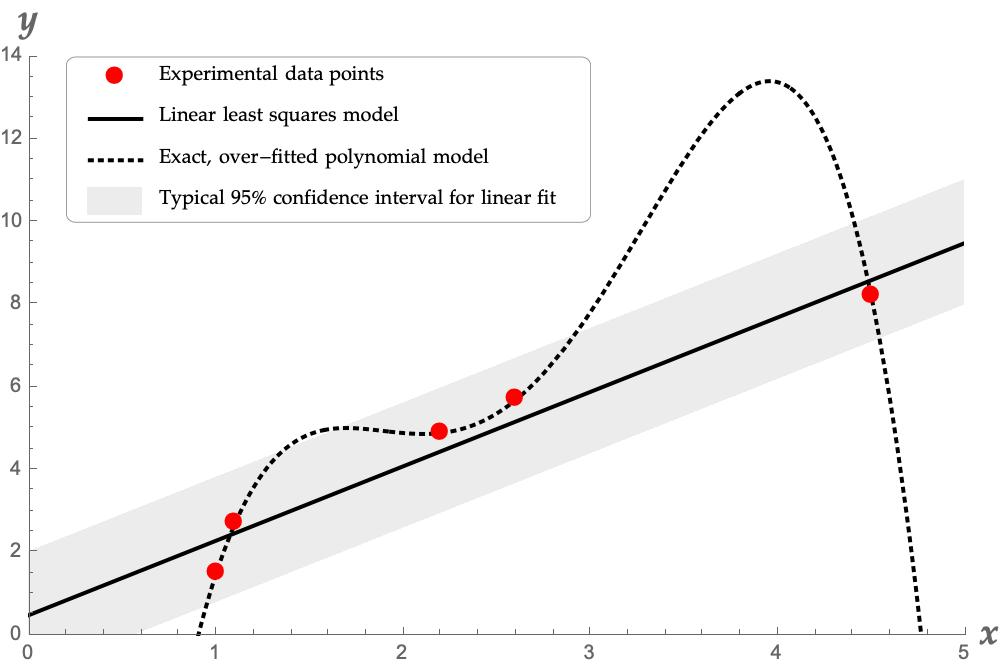
\includegraphics[width=\tw]{plot.pdf} 
%DIF < \end{change} }  
%DIF < \input generated-modelsAt5.tex
%DIF < \caption{%
%DIF < Much computational science is concerned with finding plausible multi-dimensional models that fit data. Shown here is notional experimental 2D data (the dots), together with a linear regression and an exact polynomial model. The over-fitted polynomial model fits the sample exactly, but since the experimental data is presumably subject to error (indicated by the confidence interval, itself estimated from another model) the linear model would generally be considered a better description of the experimental results. If we assume that the error in measuring $y$ is normally distributed (or similar), the extreme values the over-fitted model predicts would be considered unlikely; for example, \exacty\ predicted by the exact model versus \lineary\ predicted by the linear model.}
%DIF < \label{fig-overfit}
%DIF < \end{figure}
\DIFdelbegin %DIFDELCMD < 

%DIFDELCMD < \ignore{\subsection{Suggestions for further work}
%DIFDELCMD < Although this study of Software Engineering in scientific research (specifically, in peer reviewed publications) was necessarily interpretive in nature, the corpus of data (namely, the selected \the\dataN\ papers) was rigorously gathered so that it could be later updated or extended in size or scope. However, the insights appear to be general.
%DIFDELCMD < 

%DIFDELCMD < Further work to extend the scope of the survey beyond the basic requirements of the present paper is of course worthwhile, but the following cases (listed in the next few paragraphs) suggest that the problem is widespread. We argue, then, that we should be focusing effort on avoiding problems and considering proposed solutions (see section \ref{summary}), not just assessing the problems highlighted in this paper with increasing scale or rigor. }
%DIFDELCMD < \end{change}
%DIFDELCMD < 

%DIFDELCMD < %%%
\DIFdelend \section{Conclusions}
\DIFdelbegin \DIFdel{We need to improve the quality of code and Software Engineeringthat supports science. While this paper was originally motivated by Ferguson's public statements [], the wider evidence reviewed shows that current coding practice makes for poor science in many fields. 
}\DIFdelend In a pandemic, \DIFdelbegin \DIFdel{scientific modeling, such as epidemiological modeling }\DIFdelend \DIFaddbegin \DIFadd{epidemiological modeling (discussed in this paper)}\DIFaddend , track and trace \cite{excel-fiasco}, modeling \DIFdelbegin \DIFdel{COVID }\DIFdelend mutation pressures against vaccine shortages and delays between vaccinations \cite{science-delays}, \DIFdelbegin \DIFdel{etc}\DIFdelend \DIFaddbegin \DIFadd{and so on}\DIFaddend , drive public policy and have a direct impact\DIFdelbegin \DIFdel{on }\DIFdelend \DIFaddbegin \DIFadd{, whether positively or negatively, on the }\DIFaddend quality of life. \DIFdelbegin \DIFdel{Unfortunately, Software Engineering good practice, to help }\emph{\DIFdel{do\/}} %DIFAUXCMD
\DIFdel{science has been absent to date}\DIFdelend \DIFaddbegin \DIFadd{While this paper was originally motivated by Ferguson's public statements []
about his high-profile COVID modeling, the wider evidence reviewed here indicates that scientific coding practice is inadequate in every field. As science becomes more and more reliant on computers, we need to correspondingly improve the quality of code, the quality of code policies, the quality of Software Engineering, and the quality of all scientists' understanding of computation and how to manage its unlimited complexity}\DIFaddend . 

The main challenges to mature \DIFdelbegin \DIFdel{computational scientific research }\DIFdelend \DIFaddbegin \DIFadd{computationally-realistic science }\DIFaddend are:

\enum=1
\begin{enumerate}\raggedright
\item 
To manage software development to reduce the unnoticed and unknown impacts of bugs and poor programming practices that \DIFdelbegin \DIFdel{papers }\DIFdelend \DIFaddbegin \DIFadd{research and publications }\DIFaddend rely on. Computer code should be explicit, accessible (well-structured, etc), and \DIFdelbegin \DIFdel{properly }\DIFdelend \DIFaddbegin \DIFadd{adequately }\DIFaddend documented. Papers should be explicit on their software methodologies, limitations and weaknesses, just as Whitty expressed more generally about the standards of science \cite{whitty}. Professional software methodologies should not be ignored.

\item 
To use computation to help make scientific processes explicit, so that they can be reproduced, scrutinized and improved. RAP is an increasingly popular way to help do some of this, but as this paper points out, RAP should be generalized to \RAPstar\ to help the computational parts of science as well, leading to a virtuous circle.

\item
To support and develop the scientific community in the professional use of computation.
\DIFaddbegin 

\item
\DIFadd{To find effective ways to promote professional software engineers being recognized and participating  fully in scientific research, like professional statisticians routinely support quality research.
}\DIFaddend \end{enumerate}

While programming seems easy, and is often taken for granted and done casually, programming \emph{well\/} is very difficult \cite{fixit}. We know from software research \DIFdelbegin \DIFdel{than }\DIFdelend \DIFaddbegin \DIFadd{that }\DIFaddend ordinary programming is very buggy and unreliable. Without adequately specified and documented code and data, research is not open to scrutiny, let alone proper review, and its quality is suspect. Some have argued that availability of code and data ensure research is reproducible, but that is na\"\i ve criterion: computer programs are easy to run and reproduce results, but being able to reproduce something of low quality does not \DIFaddbegin \DIFadd{magically }\DIFaddend make it more reliable \cite{reproducibility,relit,popper-conjectures-refutations}. 

Software Engineering Boards\DIFdelbegin \DIFdel{(as introduced }\DIFdelend \DIFaddbegin \DIFadd{, as proposed }\DIFaddend in this paper\DIFdelbegin \DIFdel{) are a straight forward, constructive }\DIFdelend \DIFaddbegin \DIFadd{, are an initial, straightforward, constructive, }\DIFaddend and practical way to support and improve computer-based science. 
\DIFaddbegin 

\DIFaddend This paper's \supplement\ summarizes \DIFdelbegin \DIFdel{the relevant professional Software Engineering }\DIFdelend \DIFaddbegin \DIFadd{relevant Software Engineering good }\DIFaddend practice that Software Engineering Boards would \DIFdelbegin \DIFdel{use}\DIFdelend \DIFaddbegin \DIFadd{draw on}\DIFaddend , including discussing how and why Software Engineering helps improve code reliability, dependability, and quality.

\makeatletter
\immediate\write\@auxout{\string\def\string\continueSectionNumbers{\arabic{section}}}
\makeatother

\section*{Supporting information}
\newcount\csrefcount \csrefcount=0
\def\csref{\global\advance\csrefcount by 1}
\long\def\ethics#1{\paragraph*{Ethics}#1}
\long\def\ack#1{\paragraph*{Acknowledgments}#1}
\long\def\dataaccess#1{\paragraph*{Data and code access}#1}
\long\def\aucontribute#1{\paragraph*{Author contribution}#1}
\long\def\competing#1{\paragraph*{Competing interests}#1}
\long\def\funding#1{\paragraph*{Funding}#1}

\DIFdelbegin %DIFDELCMD < \ack{The author is very grateful for comments from: \csref Ross Anderson, \csref Nicholas Beale, \csref Ann Blandford, \csref Paul Cairns, \csref Rod Chapman, \csref Jos\'e Corr\'ea de~S\`a, \csref Paul Curzon, \csref Jeremy Gibbons, \csref Richard Harvey, \csref Will Hawkins, \csref Ben Hocking, \csref Daniel Jackson, \csref Peter Ladkin, \csref Bev Littlewood, \csref Paolo Masci, Stephen Mason, \csref Robert Nachbar, \csref Martin Newby, \csref Patrick Oladimeji, \csref Claudia Pagliari, \csref Simon Robinson, \csref Jonathan Rowanhill, \csref John Rushby, \csref Susan Stepney, Prue Thimbleby, \csref Will Thimbleby, \csref Martyn Thomas, and \csref Ben Wilson provided very helpful comments.}
%DIFDELCMD < %%%
\DIFdelend \DIFaddbegin \ack{The author is very grateful for comments from: \csref Ross Anderson, \csref Nicholas Beale, \csref Ann Blandford, \csref Paul Cairns, \csref Rod Chapman, \csref Jos\'e Corr\'ea de~S\`a, \csref Paul Curzon, \csref Jeremy Gibbons, \csref Richard Harvey, \csref Will Hawkins, \csref Konrad Hinsen, \csref Ben Hocking, \csref Daniel Jackson, \csref Peter Ladkin, \csref Bev Littlewood, \csref Paolo Masci, Stephen Mason, \csref Robert Nachbar, \csref Martin Newby, \csref Patrick Oladimeji, \csref Claudia Pagliari, \csref Simon Robinson, \csref Jonathan Rowanhill, \csref John Rushby, \csref Susan Stepney, \csref Isaac Thimbleby, \csref Prue Thimbleby, \csref Will Thimbleby, \csref Martyn Thomas, and \csref Ben Wilson. The author also thanks the anonymous \emph{Computer Journal\/} referees who also contributed to the quality of this paper.}
\DIFaddend %\the\csrefcount\ computer science reviewers.

%\ethics{This article presents research with ethical considerations but does not fall within the usual scope of ethics policies.}

\DIFdelbegin %DIFDELCMD < \dataaccess{There is an extended discussion of the methodology of this paper and its benefits in the \supplement, section \ref{on-code-data-publication}. The \supplement\ also presents all raw data in tabular form. All material is also available for download at \url{github.com/haroldthimbleby/Software-Enginering-Boards},\footnote{\color{red}This is a temporary URL before meeting publication repository requirements for accepted papers.\color{black}} which has been tested in a clean build, etc. 
%DIFDELCMD < 

%DIFDELCMD < The data is encoded in JSON\@. JavaScript code, conveniently in the same file as the JSON data, checks (with \the\JSONerrorCount\ possible classes of error report) and converts the JSON data into \LaTeX\ number registers and summary tables, etc, thus making it trivial to typeset all results reliably in this paper and in its \supplement\ \emph{directly\/} from the automatic data analysis.
%DIFDELCMD < 

%DIFDELCMD < In addition, a standard CSV file is generated from the JSON in case this is more convenient, for instance to browse directly in Excel.}
%DIFDELCMD < %%%
\DIFdelend \DIFaddbegin \dataaccess{There is an extended discussion of the methodology of this paper in the \supplement, section \ref{on-code-data-publication}. The \supplement\ also presents all raw data in tabular form. All material is also available for download at \url{github.com/haroldthimbleby/Software-Enginering-Boards},\footnote{\color{red}This is a temporary URL before meeting publication repository requirements for accepted papers.\color{black}} which has been tested in a clean build, etc. 

The data is encoded in JSON\@. JavaScript code, conveniently in the same file as the JSON data, checks (with \the\JSONerrorCount\ possible classes of error report) and converts the JSON data into \LaTeX\ number registers and summary tables, etc, thus making it trivial to typeset all results reliably in this paper and in its \supplement\ \emph{directly\/} from the automatic data analysis.

In addition, a standard CSV file is generated from the JSON in case this is more convenient, for instance to browse directly as a spreadsheet or to import easily into other programs.}
\DIFaddend 

\DIFdelbegin %DIFDELCMD < \aucontribute{Harold Thimbleby is the sole author. An preliminary outline of this paper, containing no supplementary material or data, was submitted to the UK Parliamentary Science and Technology Select Committee's inquiry into UK Science, Research and Technology Capability and Influence in Global Disease Outbreaks, under reference LAS905222, 7 April, 2020. The evidence, which was not peer reviewed and is only available after an explicit search, briefly summarizes the case for Software Engineering Boards, but without the detailed analysis and case studies of the literature, etc, that are in the present paper. It is available to the public \cite{parliamentary-evidence,my-parliamentary-evidence}.}
%DIFDELCMD < %%%
\DIFdelend \DIFaddbegin \aucontribute{Harold Thimbleby is the sole author. An preliminary outline of this paper, containing no supplementary material or data, was submitted to the UK Parliamentary Science and Technology Select Committee's inquiry into UK Science, Research and Technology Capability and Influence in Global Disease Outbreaks, under reference LAS905222, 7 April, 2020. The evidence, which was not peer-reviewed and is only available after an explicit search, briefly summarizes the case for Software Engineering Boards, but without the detailed analysis and case studies of the literature, etc, that are in the present paper. It is available to the public \cite{parliamentary-evidence,my-parliamentary-evidence}.}
\DIFaddend 

\competing{The author declares no competing interests.}

\funding{This work was jointly supported by See Change (M\&RA-P), Scotland (an anonymous funder), by the Engineering and Physical Sciences Research Council [grant EP/M022722/1], by the Royal Academy of Engineering through the Engineering~X Pandemic Preparedness Programme [grant EXPP2021\textbackslash 1\textbackslash 186], and by Assuring Autonomy International Programme, Assuring Safe AI in Ambulance Service Triage. The funders had no involvement in the research or in this paper.}

%\nolinenumbers

{\raggedright

\DIFdelbegin %DIFDELCMD < \bibliographystyle{mysiam}
%DIFDELCMD < %%%
\DIFdelend \DIFaddbegin \bibliographystyle{revisedCompJ}
\DIFaddend \def\urlprefix{}
\initialiseBibliography{References}{1}{}

\newcount \bibitemn \bibitemn = 0
\DIFaddbegin \newcount \bibnewcolumn 

\bibnewcolumn = 112 %DIF >  bibentry number of last entry on (final) left hand column
%DIF >  Hint: set it to a very large number, so the final column is as unbalanced as it gets
%DIF >  then, if it's worth fixing the final page, lower the number to some citation on the 
%DIF >  lower part of the left hand column; this citation will then become the last in that
%DIF >  column. Hopefully the righthand column will be of equal length!
%DIF >  PS Don't forget to check there is nothing on the following page!


%DIF >  if you can't get a decent column balance, tinker with the inter-citation spacing, below
%DIF >  it currently looks like "\vskip .2ex plus 1ex minus 1ex"
%DIF >  you'll be surprised what adjusting it by only 0.1ex or less achieves after 100 citations!

\DIFaddend \let\oldbibitem=\bibitem
\DIFdelbegin %DIFDELCMD < \def\bibitem#1{\ifnum \bibitemn = 0 \else \egroup\vskip .7ex plus 1ex \fi
%DIFDELCMD < \advance \bibitemn by 1
%DIFDELCMD < \vbox \bgroup \oldbibitem{#1} }
%DIFDELCMD < %%%
\DIFdelend \DIFaddbegin 

%DIF >  calculate bib entry width
\newdimen \bibEntryWidth
\bibEntryWidth = \columnwidth
\advance \bibEntryWidth by -\columnsep

%DIF >  I haven't figured out how to make the \labelwidth etc variable - it'd be nice
%DIF >  to have it suitable for numbers up to 9, then for numbers up to 99, then up to 999
%DIF >  depending on the largest bibitem number width in the column. As it is, it's set
%DIF >  to the width of 999 for all bibitems even though it takes a while for bibitems to get 
%DIF >  up to 3 figures. Sigh

\def\bibitem#1{%
\ifnum \bibitemn = \bibnewcolumn \egroup\newpage\bgroup \fi
\ifnum \bibitemn = 0 \else \egroup \fi
\advance \bibitemn by 1
\vskip .3ex plus 1ex minus 1ex 
\leavevmode \vbox\bgroup \parshape 1 0in \bibEntryWidth 
\oldbibitem{#1}}

\DIFaddend \def\endofbibliography{ \egroup \vfill}
\DIFaddbegin 

%DIF >  the class comjnl has a minor formatting bug in the setting of labelwidth; fixed below:
\makeatletter
\def\thebibliography#1{\section*{References}\small\list
 {[\arabic{enumi}]}{\labelsep 0.5em%
\hyphenpenalty=50\itemsep=-1pt
 \settowidth\labelwidth{[0#1]}% previously too small, so added an extra digit (0)
 \leftmargin\labelwidth
\advance\leftmargin\labelsep
 \usecounter{enumi}}
 \def\newblock{\hskip .14em plus .38em minus -.1em}
 \sloppy
 \sfcode`\.=1000\relax}
\let\endthebibliography\DIFadd{=}\endlist

\def\@cite#1#2{[{#1\if@tempswa , #2\fi}]}
\def\@biblabel#1{[#1]}
\makeatother

\DIFaddend \bibliography{paper-seb-main.bib}

% Note that the supplementary material calculates how many references there are,
% because it reads in this .tex file's .aux file so that it can cite the references 
%DIF <  above with the same number sequence. 
%DIF >  using the same number sequence. 
%
%DIF <  It simple redefines \bibitem to work it out while it
%DIF >  It simply redefines \bibitem to work it out while it
% defines all the citations from the bibliography above.
%
% The same technique allows the supplementary material to have 2 more bibliographies,
% with consecutive numbering.
}

%\label{LastPage}
%save Latex register    {linenumber}
%\makeatletter
%\immediate\write\@auxout{\string\def\string\MainPaperLastLine{\arabic{linenumber}}}
%\makeatother
\end{document}

\def \allInOne {define this so we don't include header in supplemental material}
\input paper-seb-supplementary-material.tex
\end{document}

%\immediate\write\@auxout{\string \newcount \string \savedlastReferenceNumber
%\string \savedlastReferenceNumber=\the\savedlastReferenceNumber}

\end{document} 
